\documentclass[utf8,english]{gradu3}

\usepackage{graphicx} 
\usepackage{amsmath} 
\usepackage{multirow}
\usepackage{lscape}
\usepackage{booktabs} 
\usepackage{longtable}
\usepackage{tikz}
\usetikzlibrary{arrows.meta,calc,fit,positioning,scopes,matrix,%
    shapes.arrows,shapes.geometric,shapes.symbols}
\usetikzlibrary{patterns}
\usepackage{pgfplots}
\pgfplotsset{compat=1.9}
\usepackage{pgfplotstable}
\usepackage{pgf-pie}
\usepackage{float}
\usepackage{paralist}
\usepackage{csvsimple}

\usepackage{biblatex}
\usepackage[bookmarksopen,bookmarksnumbered,linktocpage]{hyperref}

\addbibresource{lahteet.bib}

\pgfplotsset{
        bubbleplot count/.style={},
        bubbleplot/.style={
                scatter,
                grid=major,
                xtick=data,
                ytick=data,
                y tick label style={
                        font=\tiny
                },
                x tick label style={
                        font=\tiny
                },
                scatter/@pre marker code/.code={%
                        \scope[%
                        mark size=#1*(sqrt(\pgfmathfloatvalueof\pgfplotspointmeta)),
                        fill=black,%
                        color=black,%
                        ]
                },
                scatter/@post marker code/.code={%
                        \node[/pgfplots/bubbleplot count,color=white]%
                        {\pgfmathprintnumber\pgfplotspointmeta};\endscope
                },
        }
}

\newcommand{\createSymbolicCoords}[3]{
        \def\ylistmacro{}%
        \pgfplotstableforeachcolumnelement{#3}\of#2\as\entry{%
                \xifinlist{\entry}{\ylistmacro}{}{%
                        \listxadd{\ylistmacro}{\entry}%
                        \edef#1{#1{\entry},}%
                }%
        }
}

\begin{document}

\title{Software development for people with intellectual or developmental disabilities in 2010--2019: \\a systematic mapping study}
\translatedtitle{Ohjelmistokehitys kehitysvammaisille henkilöille vuosina 2010--2019: systemaattinen kirjallisuuskartoitus}
\studyline{Software engineering}
\avainsanat{%
  kehitysvamma,
  autismikirjo,
  ohjelmistokehitys,
  kirjallisuuskartoitus
}
\keywords{%
  intellectual disability,
  developmental disability,
  Autism spectrum disorders,
  software design,
  software development,
  mapping study}
\tiivistelma{%
  Kehitysvammaiset henkilöt voivat tarvita ohjelmistoja, jotka on kehitetty ottamaan
  heidän vammansa huomioon.
  Vuoden 2006 Yhdistyneiden Kansakuntien vammaisten henkilöiden oikeuksia koskevan yleissopimuksen
  yhdeksäs artikla, joka koskee esteettömyyttä, tiivistää tämän tutkimuksen taustasyyt.
  Tämä pro gradu -tutkielma suoritti systemaattisen kirjallisuuskatsauksen ohjelmistoista
  kehitysvammaisille henkilöille, jotka julkaistiin tieteellisinä artikkeleina tai konferenssipapereina
  vuosina 2010--2019. Hyväk\-syttyjä artikkeleja oli 98 kappaletta.
  Tärkeimmät löydökset ovat kirjallisuuden vähäinen määrä ja lisääntyminen vuosikymmenen aikana.
  Ohjelmistojen tarkoitetut käyttäjät ovat yleisimmin lapsia, joilla
  on autismikirjon häiriö tai älyllinen kehitysvamma.
  Lähes puolet ohjelmistoista liittyivät mobiiliteknologiaan.
}
\abstract{%
  People with intellectual or developmental disabilities (IDD) may need software applications that are
  specifically developed to answer the requirements their disabilities pose.
  Article 9 of the 2006 Convention on the Rights of Persons with Disabilities of the United Nations,
  which concerns accessibility, summarizes the motivation of this study.
  This thesis conducted a systematic mapping study of applications for people with IDD
  that were published as journal articles or conference papers in 2010--2019.
  There were 98 accepted articles.
  Key findings include a rising, yet small, amount of literature through the decade.
  The intended users most popularly are children and have either
  Autism spectrum disorder or an intellectual disability.
  Nearly half of the applications had a connection to mobile technology.
}

\author{Mari Kasanen}
\contactinformation{\texttt{remasoka@student.jyu.fi}}
\supervisor{Ville Isomöttönen}

\maketitle

\mainmatter

%############################################
%                                    1. luku
%############################################
\chapter{Introduction}

Intellectual or developmental disabilities (IDD) cover a range of disabilities,
such as Autism spectrum disorders and varying intellectual disabilities,
that usually manifest in childhood and continue throughout life~\parencite[e.g.][]{dsm5}.
People with IDD have varying limitations that affect their daily lives in several ways.
They may have restricted cognitive abilities or difficulty with fine motor skills.
As a result, the software applications they use must take their needs into consideration.
Often this means that there must have been significant thought put into the accessibility
of the application during its development process, as well as efforts in understanding
and sometimes overcoming the limitations of the disability.

According to the Convention on the Rights of Persons with Disabilities (CRPD) from 2006,
States Parties shall take appropriate measures ``to promote access for persons with disabilities
to new information and communications technologies and systems, including the Internet'',
and ``to promote the design, development, production and distribution of accessible
information and communications technologies and systems at an early stage, so that these
technologies and systems become accessible at minimum cost'' \parencite[Article 9]{unitednations}.
The Finnish Association on Intellectual and Developmental Disabilities (FAIDD)
aims at enacting the articles of CRPD in Finland by giving people with IDD a voice in society.

\begin{quote}
  \centering
  \textit{``Everyone has the right to develop and learn new things \\through proper support.''}
  \begin{flushright}
    \footnotesize{---\textcite{kehitysvammaliittoID}}
  \end{flushright}
\end{quote}

The above quote and Article 9 of the CRPD summarize the societal motivation for this study.
Part of the mentioned proper support for people with IDD can be software applications
made specifically to answer their unique requirements, and to aid them in learning and living.

This thesis is conducted as a systematic mapping study, aiming to describe the spectrum
of software applications made for people with IDD.
The applications of interest are published as either journal articles or conference papers
within the decade of 2010--2019.
Providing an overview of the published scientific literature regarding these software applications
may result in finding research gaps or topic areas suitable for more focused literature reviews,
or providing people involved in the life of a disabled person with ideas
of how they may utilize information technology.

The six research questions of this thesis (see Chapter~\ref{questions})
examine when and where the applications were published as articles,
and what type of research the articles represent.
They also examine the disabilities and age groups the applications target,
as well as the platforms the applications are developed for.
The final research question regards the purposes of the software applications,
aiming to categorize the purposes and thus share a more detailed awareness of the subject area.

A limited search for similar secondary studies in January 2020 yielded
22 studies, only one of which was a mapping study~\parencite{ascari2018}.
None of the studies shared the scope of this thesis,
all of them having a more narrow scope in terms of the disabilities or
the technologies they study.
Literature reviews with more narrow focus areas seem to be the most common form of secondary study
on the subject of using information technology for the benefit of people with IDD,
which suggests that more mapping studies could be made of the area.

The rest of this thesis is structured as follows.
Simplified descriptions of the most relevant disabilities, and an overview of types
of software applications made for people with those disabilities are provided in Chapter two.
Chapter three includes a description of mapping studies as a research method
as well as decisions made regarding this thesis based on the guidelines of
\textcite{petersen2008} and \textcite{petersen2015guidelines}.
The research method of this study is described in detail in Chapter four.
Chapter five presents the systematic map as the result of this mapping study,
illustrating answers to the research questions.
Chapter six concludes this thesis with a discussion.


%############################################
%                                    2. luku
%############################################
\chapter{Intellectual or developmental disabilities and software}

Intellectual or developmental disabilities affect the development of a person,
manifest themselves before adulthood, and persist throughout the person's life~\parencite[e.g.][]{dsm5}.
IDD cover a range of disabilities that have the aforementioned things in common,
but may show varying symptoms and have different needs and limitations.
This thesis complies with the categorization that developmental disabilities include,
among others, intellectual disabilities, cerebral palsy, as well as pervasive developmental disorders,
of which the most notable within the thesis are Autism spectrum disorders.

The focus of the thesis resides in software development, but simplified descriptions
of disabilities are given to enhance and ensure the understanding of the reader.
The rest of this chapter first gives descriptions and estimates of prevalence
of the most relevant disabilities for this thesis.
Then examples of software applications made for people with IDD and the opportunities
the applications provide are reviewed.


\section{Disability descriptions and prevalence}

The most commonly mentioned disabilities within the investigated articles of this mapping study
are Autism spectrum disorders (ASD) and intellectual disabilities.
This chapter gives descriptions of the two disabilities
using diagnostic criteria provided by DSM-5 \parencite{dsm5},
the fifth edition of the Diagnostic and Statistical Manual of Mental Disorders,
and giving estimates of the number of people affected.
The end of this chapter introduces a related term, complex communication needs,
which applies to a portion of people with IDD who have communicative deficiencies.

According to~\textcite{dsm5}, the currently used diagnostic criteria for ASD entail
persistent deficiencies in social communication and social interaction, e.g. deficits in social-emotional reciprocity,
nonverbal communicative behaviors, and developing, maintaining, and understanding relationships.
The criteria also include exhibiting restricted and repetitive patterns of behavior, interests, or activities,
such as movements, speech, inflexible attachment to routines,
fixated interests with exceptional intensity, and hyper- or hyporeactivity to sensory input.
Important areas of functioning are significantly impaired by these symptoms,
which must be present in the early developmental period~\parencite{dsm5}.
ASD is not considered a degenerative disorder, and people with ASD typically
continue to learn throughout their lives, but an individual  with severe symptoms
might never live and work independently~\parencite{dsm5}.

Reported frequencies for ASD have approached 1\% of the population~\parencite{dsm5},
and based on this estimate, Finland would have an estimated 55 000 people with ASD~\parencite{autismiliitto}.
\textcite{baio2018} reported on the Autism and Developmental Disabilities Monitoring Network,
including 11 sites across the United States that monitor 8-year-old children for ASD,
and in 2014 the prevalence of ASD was 1.68\% (1.31--2.93\% among the 11 sites).
They noted that the estimate prevalence of 2014 is higher than the network's previous estimates,
and that the estimate has continuously increased from the estimate in 2000, which was 0.67\%~\parencite{baio2018}.
The rising prevalence rates might reflect an actual increase in the frequency of ASD, but a combination
of reflecting usage of the previous diagnostic criteria of DSM-4, increased awareness,
and differences in study methodologies~\parencite{dsm5}
may account for the rise as well.

Possible causes for intellectual disability include genetic factors, problems or alcohol use during pregnancy,
lack of oxygen at birth, childhood injury, and childhood illnesses~\parencite{kehitysvammaliittoID}.
According to \textcite{dsm5}, intellectual disability onsets during the developmental period,
and affected individuals exhibit deficits in intellectual and adaptive functioning.
The deficits in intellectual functions affect for example problem solving, abstract thinking, and learning,
while deficits in adaptive functioning result in ``failure to meet developmental and sociocultural standards
for personal independence and social responsibility''~\parencite{dsm5}.
The \textcite{kehitysvammaliittoID} estimates that around 40 000 people have an intellectual disability in Finland,
while a global estimate of prevalence in the general population is approximately 1\%~\parencite{dsm5}.
Intellectual disability is generally nonprogressive, not including specific genetic disorders with
periods of worsening or progressive worsening of intellectual function~\parencite{dsm5}.
People with profound intellectual disabilities or multiple disabilities need continuous support,
but in mild cases the person might cope relatively independently~\parencite{kehitysvammaliittoID}.

While intellectual disability and ASD are separate disorders, they can manifest comorbidly.
A study in the state of South Carolina examined the prevalence of ASD among children with intellectual disability.
They found that the prevalence was 18.04\%, while ASD rates for the general South Carolina
population were reportedly 0.60--1.11\%~\parencite{tonnsen2016}.

Another term that applies to many people with IDD is \textit{complex communication needs} (CCN).
While not a diagnosis, CCN refers to people who have difficulty producing or understanding speech,
making them unable to cope in everyday communication situations by speech alone~\parencite{kehitysvammaliittoCCN}.
People with CCN may benefit from augmentative and alternative communication (see Chapter~\ref{softat}).
The \textcite{kehitysvammaliittoCCN} estimates that of the 65 000 people with communicative impairments in Finland,
30 000 need augmentative and alternative communication.


\section{Software development for people with IDD} \label{softat}

Depending on their disability, their symptoms and severity,
a person with IDD needs support that varies in type and intensity.
The specific needs and requirements of people with IDD may also
be hard to attain, due to difficulties in communication.
For example, people with severe Autism can be unable or unwilling
to participate in assessments~\parencite{holt2014},
and therefore even with the help of a disabled user
a software developer with no previous knowledge
of the disability could be unable to develop an application
that sufficiently answered the needs of the user.
While society shifts towards using an increasing amount of information technology,
users with disabilities face possible exclusion~\parencite{dekelver2015}.
Therefore those developing the applications must consider users with disabilities.

Assistive technologies have been shown to have advantages,
such as lasting benefit of memory exercises, easier adoption of technology through electronic means
and a feeling of being more independent~\parencite{dekelver2015}.
Specifically the use of mobile devices by people with IDD or complex communication needs has been studied.
A review of studies with developmentally disabled people using touchscreen mobile devices
found that touchscreen use had reportedly positive effects~\parencite{stephenson2015}.
Increased adoption as well as increased awareness and social acceptance
were benefits that \textcite{mcnaughton2013} highlighted for the field of
augmentative and alternative communication (AAC) using mobile technology.

\textcite{line2018} give recommendations regarding game design
when the user has deficits in mental abilities, communication,
coordination, learning, attention, or social interaction.
The primary focus of their study is hypersensitivity to sounds
in neurodevelopmental disorders, and they propose strategies such
as gradual sound exposure to counteract the sensitivity.
\textcite{dekelver2015} also list design recommendations,
but for mobile user interfaces for people with IDD.
They include pieces of advice such as ``The size of `clickable' areas should be increased''
and ``Warnings and feedback should stay on the screen as long as the user does not
respond to them'', while also encouraging using high contrast between
text and background and avoiding cognitive overload by limiting the
number of functions~\parencite[p. 829]{dekelver2015}.

Some of the areas that software applications for people with IDD
confront are communication, therapy, and training of various skills.
The rest of this chapter gives examples of applications within those
categories, in the order they were mentioned.
Skill training is further divided into the training of cognitive skills,
life skills, and emotional or social skills.

Many people with IDD have communicative deficits, as reflected by the diagnostic criteria
for ASD and intellectual disability~\parencite{dsm5}.
AAC aims to enable all people to communicate~\parencite{ascari2018}, and as such it may benefit people with IDD.
Ranging from physical photo cards to electronic communication boards and voice synthesizers~\parencite{ascari2018},
AAC devices offer many digital and analogue alternatives.
PECS (Picture Exchange Communication System), an analogue AAC system,
was developed for children with ASD, and its roots combine AAC guidelines
and applied behaviour analysis (ABA) principles~\parencite{de2011}.
With the analogue PECS, a set of laminated picture cards is used which are kept in a binder, but
managing and maintaining images in an analogue communication system
may grow difficult as the child's vocabulary grows~\parencite{de2011}.
Digital communication boards have emerged,
and two examples include Araboard by \textcite{baldassarri2014}
and PixTalk by \textcite{de2011}.
Both of these applications may be used with a mobile device for easy inclusion into daily activities,
and they both provide a separate software tool for creating or editing the communication boards.
This means a guardian or teacher of a disabled person may create personalized communication boards
tailored for the disabled individual and the situations they encounter.

The following examples of therapy applications all offer a digital alternative
to an analogue form of therapy that has been shown to be effective.
\textcite{artoni2018technology} present an application for ABA intervention,
aimed at children with Autism.
The application is used on a tablet device, with no real objects which reduces set up time,
and the application records the child's performance and helps with analyzing it~\parencite{artoni2018technology}.
\textcite{barate2018} present a music therapy application using the Leap Motion controller,
which interprets hand motions in the air and converts them into presses on the application.
The user interface on this software application is vertically divided into (two or more) rectangular areas
that produce sounds with different pitches when pressed.
The application is aimed at people with intellectual or motor disabilities, providing them with a
way of participating in creating music despite motor challenges.
Virtual reality (VR) therapy applications may make some forms of therapy, such as dolphin-assisted therapy, more accessible.
Dolphin-assisted therapy has reported benefits in attention, motor skills, and nonverbal communication,
but a VR version may increase its availability and affordability~\parencite{cai2013}.
Another VR therapy application by~\textcite{poyade2019isensevr} delivers exposure therapy.
The application involves a scenario in an airport environment, designed to increase the user's
tolerance of heightened noises and crowded situations.

Training cognitive skills such as attention, memory, or task switching can be done with software applications.
The following examples are all developed as games for intellectually disabled users to attain or improve cognitive skills.
\textcite{bargagna2014} present a learning game to provide telerehabilitation of cognitive skills for adults with Down syndrome,
who may be at a great risk of dementia due to showing a susceptibility to Alzheimer's disease.
In their game the user is faced with increasing difficulty levels according to their previous activity.
Telerehabilitation may improve access to care for some patients~\parencite{bargagna2014}.
\textcite{robb2019} present a training game for the skill of task switching for children with Prader-Willi syndrome.
An educational memory game by \textcite{segatto2017} for intellectually disabled people
has three difficulty levels, of which the appropriate level must be chosen according to the player's cognitive level.
They propose the cognitive level to first be evaluated by a therapist.

The application examples that teach life skills to users with IDD
involve self-care through eating and hygiene,
and independence through public transport and work skills.
\textcite{hatzi2015} presents a cartoon-style serious game for teaching healthy eating
for adolescents with Down syndrome, using simple-layout stages for minimizing cognitive load.
A motion-controlled game by \textcite{kang2019} for intellectually disabled children aims to teach hand hygiene.
\textcite{rezae2019} present a tool for planning public transport routes for users with ASD,
as safety and spatial awareness are prevalent concerns among Autistic individuals and their families.
The users may also need help with managing anxiety or sensory sensitivity while using public transport.
\textcite{tsiopela2017} present a learning environment for students with ASD for improving pre-vocational skills
such as attention to details, preparedness, self-evaluation, and familiarization with objects and working routines.
The environment offers opportunities to practice,
but practice in a realistic context should be incorporated~\parencite{tsiopela2017}.

The following examples of training emotional or social skills are all aimed at people with ASD,
as they often have difficulty with these particular skills.
A role-playing game for recognizing basic emotions by \textcite{almeida2019}
applies attractive illustrations and multisensory feedback to help maintain the user's attention.
\textcite{ip2018} present a VR application with learning scenarios for emotion control and relaxation strategies
and simulations for social situations. Their application enables repeated practice in scenarios
that in a real environment would not be easily organized for repetition.
A collaborative game for facilitating other-awareness is presented by \textcite{holt2014}.
Their ``separate control of shared space'' game enables low-functioning children with Autism
to present other-awareness in specific situations.

Broadly summarizing these example applications,
many AAC and therapy applications aim to digitize previously used analogue methods,
while skills are often taught using games.
Accommodating the cognitive skills of a person with IDD by for example
considering how information is delivered, and
obtaining and maintaining the attention of the user
are key problems to solve during development of these applications.


%############################################
%                                    3. luku
%############################################
\chapter{Systematic mapping study} \label{mapping}

A mapping study can identify research gaps or indicate a lack of a certain type
of research within a topic area~\parencite{petersen2008}.
This chapter offers an overview of the method of a systematic mapping study,
as provided by \textcite{petersen2008} and the updated guidelines of \textcite{petersen2015guidelines}.
Brief comparisons of the general method to conducting this thesis are made,
while Chapter~\ref{method} depicts these matters with more detail.
The subchapters examine more closely the categorization of the accepted articles,
and the similarities and differences between mapping studies and literature reviews.

Table~\ref{mappingtable} shows the systematic mapping process as \textcite{petersen2008} presented.
The process consists of five steps, each having its own outcome.
In this thesis the steps were adhered to as follows.
After defining research questions and conducting searches, 2978 papers were found.
These papers were then screened in two phases (details in Chapter~\ref{searches}).
The first phase found 159 potential papers, of which the second phase eliminated a further 61 papers,
leaving the total of accepted papers at 98. Appendix~\ref{appendixA} lists the accepted papers,
and appendix~\ref{appendixB} lists the potential papers that were excluded during the second phase.

\begin{table}[h]\centering
  \begin{tabular}{|p{6.5cm}|p{4cm}|}
    \hline
    \textbf{Process steps}              & \textbf{Outcomes}     \\ \hline
    Definition of research questions    & Review scope          \\ \hline
    Conduct search                      & All papers            \\ \hline
    Screening of papers                 & Relevant papers       \\ \hline
    Keywording using abstracts          & Classification scheme \\ \hline
    Data extraction and mapping process & Systematic map        \\ \hline
  \end{tabular}
  \caption{Systematic mapping process by \textcite{petersen2008}}
  \label{mappingtable}
\end{table}

The fourth step of the mapping process is keywording. This began during the third step of paper screening,
with writing down potential answers to research questions as well as other important pieces of information.
The fourth and fifth steps were alternated between several times, as the keywording was conducted separately
for each research question before the final data extraction.
\textcite{petersen2015guidelines} note that the mapping process is iterative,
and the process may require revisions during the mapping.
The final outcome of the process, the systematic map, is presented in Chapter~\ref{results}.

Even though the fourth step is called ``keywording using abstracts,'' \textcite{petersen2008} state that
\enquote{abstracts are often misleading and lack important information,} instead advocating for
allowing more detailed study of papers when the abstract does not provide all needed information.
Considering more parts of a paper requires more effort, but also increases the validity of results~\parencite[p. 9]{petersen2008}.
This thesis examined all accepted articles at least once for each research question,
studying also introductions, conclusions and other parts of papers, as necessary.

The reporting of this study follows quite closely the structure that \textcite{petersen2015guidelines} suggest
while also satisfying the conditions of a Master's thesis. The second chapter of this thesis is not called ``related work''
as suggested, but nevertheless aims to provide a scientific theoretical base for this study.
This thesis also divides into two parts the suggested ``research method'' chapter,
focusing in this chapter on mapping studies in general,
while Chapter~\ref{method} presents details on how this study was conducted, specifically.

\textcite{kitchenham2011} note potential problems with mapping studies, such as insufficient rigor, as well as
time and effort restrictions especially when a mapping study is conducted by a Master's student, like in the case of this thesis.
Conducting a mapping study by oneself imposes obvious risks to the validity of the study, but
Chapter~\ref{method} describes the method and Chapter~\ref{results} the results in an effort to convince
the reader of the rigor and relevancy of this thesis.

\section{Categorizing the papers} \label{classified}

The papers are divided into topic-independent categories based on types of research.
Consistent use of similar classification schemes
enables comparisons between different mapping studies \parencite{petersen2015guidelines}.
As proposed by \textcite{petersen2008}, this thesis uses a classification system by \textcite{wieringa2006requirements}.
The six categories are explained in Table~\ref{classes}. Due to this thesis' focus on papers that present or evaluate a
software application, categories such as \textit{philosophical papers}, \textit{opinion papers} or
\textit{personal experience papers} should not have prevalence, although they are not explicitly excluded.

\begin{table}[h]
  \centering
  \begin{tabular}{|p{3.5cm}|p{9cm}|}
    \hline
    \textbf{Category}          & \textbf{Summary}                                                                                                                                                                                            \\ \hline
    Evaluation research        & Investigates a problem or an implementation of a technique in practice.                                                                                                                                     \\ \hline
    Proposal of solution       & Proposes a solution while arguing for its relevance without complete validation. The technique must be novel or a significant improvement of an existing technique.                                         \\ \hline
    Validation research        & Investigates properties of a solution proposal that has not previously been implemented in practice. The solution may have been proposed elsewhere. Uses a thorough, methodologically sound research setup. \\ \hline
    Philosophical papers       & Introduces a new way of looking at things, e.g. a new conceptual framework.                                                                                                                                 \\ \hline
    Opinion papers             & Offers the author's opinion about what is wrong/good about something, how something should be done, etc.                                                                                                    \\ \hline
    Personal experience papers & Emphasizes what has happened, instead of why. Lists lessons learned by the author from their experience. Experience is reported without a discussion of research methods, and evidence can be anecdotal.    \\ \hline
  \end{tabular}
  \caption{Classification system by \textcite{wieringa2006requirements}}
  \label{classes}
\end{table}

Papers can belong to more than one category \parencite{wieringa2006requirements}.
In this thesis, each paper was nevertheless assorted into a single category.
While \textcite{petersen2008} found these categories easy to interpret and use,
\textcite{petersen2015guidelines} mentioned that researchers were not always consistent
in their classification when using them. The distinction between evaluation and validation research
that \textcite{petersen2015guidelines} use is that validation is done in a laboratory environment,
while evaluation takes place in a real world context.
This distinction was also adopted for use in this thesis.
When a study did not report where their experiment was held,
the place was assumed to have been a laboratory environment.
In the case that laboratory tests and real world tests were both reportedly conducted,
the study was assorted as evaluation research.


\section{Mapping studies and literature reviews}

Systematic mapping studies and systematic literature reviews (SLR) have many similarities, but also key differences.
Both methods are forms of secondary research, aggregating prior primary research.
In software engineering, the systematic mapping study process, as described by \textcite{petersen2008},
and the systematic literature review process, as described by \textcite{kitchenham2009},
are similar in the beginning, starting with posing research questions,
formulating the criteria for inclusion and exclusion, and conducting the search for literature.
The methods differ in their goals, breadth and depth, and should be used complementarily~\parencite{petersen2008}.

While both methods define research questions, \textcite{kitchenham2011} describe the research questions
for a mapping study as ``high level'' and those for an SLR as ``very specific'', and state that
mapping studies also often have more research questions than SLRs.
The methods also clearly diverge toward the ends of the processes, as primary studies are treated differently.
SLRs review a smaller amount of studies in-depth, requiring considerable effort,
and mapping studies review a larger amount of studies with less detail~\parencite{petersen2008}.
Mapping studies generally do not aggregate the outcomes of primary studies~\parencite{kitchenham2011}.

Mapping studies aim to provide an overview of a topic area, and the knowledge gained can be used
to find a suitable topic to conduct an SLR~\parencite{petersen2008, kitchenham2011}.
Even though their goals are different, there can be an overlap between the methods~\parencite{kitchenham2011}.
\textcite{petersen2008} offer a viewpoint of considering the methods as different points in a continuum:
a mapping study may gain SLR traits by delving deeper into the papers, and an SLR may benefit of a more
quantitative approach or visualization techniques characteristic to a mapping study.

This thesis has multiple research questions which are answered graphically. It also has a broad topic.
Research questions 3--6 (see Chapter~\ref{questions}) are more specific than the first two,
and answering them requires more detailed study of the accepted papers.
Thus this thesis is a mapping study with some deeper study of papers.


%############################################
%                                    4. luku
%############################################
\chapter{Research method} \label{method}

A search for similar secondary studies was conducted in September 2019, and an updated search in January 2020.
The digital repository of the University of Jyväskylä, JYX, contained no mapping studies or literature reviews on the subject.
Searches with Scopus and Google Scholar found 22 similar or related studies, and they are listed in Appendix~\ref{appendixD}.
Only one of the found secondary studies \parencite{ascari2018} is a mapping study,
and it focuses on mobile interaction for augmentative and alternative communication.
The scopes of all found studies are more narrow than the scope of this thesis either in terms of the disability or
the technologies they study.
Therefore it was concluded that no mapping study of this scope had been published before.

This chapter gives detailed information on how this thesis was conducted as a systematic mapping study.
The results form a systematic map of scientific literature that showcases and/or evaluates
software applications made specifically for intellectually or developmentally disabled users.
The systematic map can be found in Chapter~\ref{results}.
The subchapters introduce the research questions and inclusion criteria, describe the literature searches,
show the amount of found literature, and present how information was extracted from the papers.

\section{Research questions} \label{questions}

In the center of this thesis are software applications for intellectually or developmentally disabled users.
This thesis aimed to study scientific literature published about these applications and
then provide an overview of them, with the help of the following questions:

\begin{enumerate}
  \item When and where has the subject been studied?
  \item What kinds of studies were they?
  \item Which disabilities do intended users of the applications have?
  \item What age are intended users of the applications?
  \item What platforms are the applications developed for?
  \item What are the purposes of the applications?
\end{enumerate}

The first two questions give topic-independent insight into the research area as a whole.
The first question is answered by sharing publication years and forums of the articles, and
the second by classifying the articles by type of research, with a classification system (see Chapter~\ref{classified})
by \textcite{wieringa2006requirements}.

Questions three and four focus on intended users of the applications.
As answers, the distribution of articles by the relevant categories are shown.
The fifth question divides the applications into five platforms listed in Chapter~\ref{criteria}.
The answer to the sixth and last question lists what the software applications aim
to achieve or what their primary purposes are.

\section{Inclusion criteria} \label{criteria}

Any piece of accepted literature in this thesis should be:
\begin{itemize}
  \item presenting and/or evaluating a software application developed for intellectually or \\developmentally disabled users, developed for the platform of augmented reality, \\mobile, personal computer, virtual reality, or web,
  \item available either for free or as a member of the University of Jyväskylä,
  \item available as a whole in a digital form,
  \item published in 2010--2019,
  \item written in English, and
  \item a peer-reviewed journal article or conference paper.
\end{itemize}

In order to regard a software application as developed for intellectually or developmentally disabled users,
people with a disability that is relevant to this thesis must be mentioned either as the intended
users or testers. The intended users may include groups other than people with these disabilities.
The application must be intended to be operated by a disabled user.
It must be apparent in the study that developing the application requires programming.

A piece of literature is excluded if it is a book, a thesis, a duplicate, or only partially available digitally.
Also studies that clearly use a ready-made robotic device or present more than one software application are excluded.
In case of finding multiple studies reporting on the same application, only one of those studies is included.

\section{Literature searches} \label{searches}

This chapter introduces the search terms and search engines that were used,
as well as how all found literature was processed to arrive at the accepted articles of this study.

The used search terms comprised two parts: the relevant disabilities, and a connection to producing software.
Two different search terms were used, and they can be found in Table~\ref{termit}.
The first search term is more restrictive with producing software,
and it was used with search engines that aggregate results from multiple places (ProQuest, Google Scholar).
The second search term is less restrictive, only requiring a mention of the word ``software'',
and it was used with non-aggregating search engines (IEEE Xplore, ACM), as well as Scopus.
With Scopus, several additional limitations were added to the search (see Table~\ref{table}),
and thus using a less restrictive search term yielded a reasonable number of search results.

\begin{table}[h!]
  \centering
  \caption{Search terms}
  \label{termit}
  \begin{tabular}{|p{0.1\linewidth}|p{0.7\linewidth}|}
    \hline
    \textbf{\#} & \textbf{Logical search term}                                                                                                                                                                                                                  \\ \hline
    1           & (``intellectual disability'' OR ``intellectual disabilities'' \newline OR ``developmental disability'' OR ``developmental disabilities'') \newline AND (``software design'' OR ``software engineering'' \newline OR ``software development'') \\ \hline
    2           & (``intellectual disability'' OR ``intellectual disabilities'' \newline OR ``developmental disability'' OR ``developmental disabilities'') \newline AND (``software'')                                                                         \\ \hline
  \end{tabular}
\end{table}

Preliminary searches were performed on several search engines selected from a list provided by
the library of the University of Jyväskylä.
The used search engines are ones that entailed relevant content during preliminary searches and the engines are listed
as part of Table~\ref{table}. The table also indicates which search term was used,
when the search was conducted, and what engine-specific limitations were applied.
The searches were conducted between September 24th and November 4th of 2019.
In addition, Table~\ref{table} portrays the total number of search results from each search engine,
the numbers of potential and accepted articles, as well as percentages of accepted articles versus total results.
The highest percentage of accepted articles from a search engine is 51.85\% (IEEE Xplore),
and lowest 2.15\% (Google Scholar).


\clearpage
\begin{landscape}
  \begin{table}[p]
    \caption{Literature searches and their results}
    \label{table}
    \begin{tabular}{|l|p{0.075\linewidth}|l|p{0.25\linewidth}|p{0.065\linewidth}|p{0.075\linewidth}|p{0.075\linewidth}|p{0.095\linewidth}|}
      \hline
      \textbf{Search engine} & \textbf{Search term*} & \textbf{Date}     & \textbf{Additional limitations}                                                                                                            & \textbf{Total results} & \textbf{Potential results} & \textbf{Accepted results} & \textbf{Accepted results (\%)} \\ \hline
      ProQuest               & 1                     & Sept. 24 - 25     & Limit to: full-text, peer-reviewed. Source type: conference papers \& proceedings, scholarly journals.                                     & 245                    & 28                         & 16                        & 6.53\%                         \\ \hline
      IEEE Xplore            & 2                     & Sept. 25          & -                                                                                                                                          & 27                     & 19                         & 14                        & 51.85\%                        \\ \hline
      ACM                    & 2                     & Sept. 30          & ACM Full-Text Collection                                                                                                                   & 10                     & 2                          & 1                         & 10.00\%                        \\ \hline
      Scopus                 & 2                     & Oct. 1            & Search from: title, abstract, and keywords. Subject area: Computer Science. Document type: article or conference paper. Language: English. & 67                     & 18                         & 9                         & 13.43\%                        \\ \hline
      Google Scholar         & 1                     & Oct. 4 - Nov. 4   & No patents, no citations.                                                                                                                  & 2629\textbf{**}        & 92                         & 58                        & 2.15\%                         \\ \hline
      \textbf{All}           &                       & Sept. - Nov. 2019 &                                                                                                                                            & \textbf{2978}          & \textbf{159}               & \textbf{98}               & \textbf{3.29\%}                \\ \hline
    \end{tabular}
    * = complete search terms in Table~\ref{termit}

    ** = number of results that were shown and inspected
  \end{table}
\end{landscape}
\clearpage

The search for literature was conducted in two distinct phases.
The first phase processed 2978 results from five different search engines.
The results were inspected and graded \textit{yes, maybe,} or \textit{no}
based on how the article met the inclusion criteria.
In Table~\ref{table}, ``potential results'' refers to
articles graded either yes or maybe during this phase.

With Google Scholar the searches were carried out one year at a time, starting from 2019 and ending at 2010.
This was done to circumvent the search engine's feature to only show up to 1000 results at once.
The same search term and additional limitations were used each time, only the start and end year of the search were altered.
In hindsight, a more fitting search term should have been formulated for Google Scholar to reduce the
number of search results and to prevent redundant work.

It should be noted that on Google Scholar the number of results that was presented at the beginning of a search
frequently did not match the number of results that were shown.
At most, the number of shown and therefore inspected results was 11 fewer or 26 more
than the presented number. Contemplating the features of a search engine is not in the scope of this
thesis. A decision was made to only express the number of results
that were inspected (see Google Scholar in Table~\ref{table}).

In the second phase of the literature searches, the 159 potential articles were re-reviewed.
At this time, a list of thirteen potential papers was given to the supervisor of this thesis,
who reviewed them and provided opinions. The inclusion criteria were sharpened as a result.
Literature searches on ProQuest, IEEE Xplore, ACM and Scopus were all conducted with no time limits,
which led to a total of six potential articles being excluded in the second phase for being published before 2010.

For a potential article to become accepted, it needed to fulfill all the inclusion criteria.
Publication Forum\footnote{https://www.tsv.fi/julkaisufoorumi/haku.php}
was used for checking the publications for their peer-review process or lackthereof.
Publication Forum grades publications from levels 0 to 3, higher being more prestigious, and
reaching level 1 requires the publication to be peer-reviewed. Publications that were graded
as 0 or were not found on Publication Forum, were manually investigated on the web.
If a forum did not have a mention about peer-reviewing their content or give indication
of a review or selection process, its articles were excluded.

Also during the second phase, some papers were excluded for reporting on the same software as other articles.
Eight software were found to identifiably have multiple papers about them, and the extra papers were excluded.
The included article was decided based on how well the result showcased the software, and how far along the
development process was at the time of writing. In many cases this meant including the latest article.
In one case there were multiple papers of the same project, which spanned many years.
Two different articles were included from the project, because even though the purpose of the applications was the same,
the first application was clearly a mobile application for Android~\parencite{artoni2013portable},
and the latter a web application~\parencite{artoni2018technology}.
After the second phase, a total of 98 articles were accepted.


\section{Data extraction}

Information of all search results was gathered into a spreadsheet file,
which was stored in a private version control repository.
Each result comprised a single row of the file, with columns for used search engine,
grade of meeting inclusion criteria, bibliographical information and answers to research questions.
Potential articles were downloaded as pdf files, and subsequent examination of the articles
took place via the pdf files and the spreadsheet file.

Initial answers to the research questions were documented during both phases of
the literature searches for potential articles.
After the second phase, final answers to the research questions were extracted.
The final extractions were attained one question at a time by examining all of the
accepted articles within the context of the research question.
Answers were written down in the spreadsheet file, and then compared with each other,
leading to categorizations when the question demanded it.
Extracting answers to research questions 3--6 warranted more detailed
study of the papers. All parts of papers were considered when necessary.


%############################################
%                                    5. luku
%############################################
\chapter{Results} \label{results}

Figure~\ref{kuvaOtsikot} presents a wordcloud\footnote[2]{Made with www.wordclouds.com. The titles were
  unified beforehand  in terms of capital/lowercase letters and spelling of specific disabilities. Phrases that were
  mentioned less than three times and generic verbs (e.g. ``use'') were eliminated.} of the titles of included results,
aiming to give the reader an initial understanding of their contents.
The word ``children'' was the most frequent one, mentioned in roughly half of the titles.
The focus of this study is on \textit{intellectual disability} and \textit{developmental disability},
and they are also the phrases used as search terms during literature searches.
Despite this, three specific disabilities arise in the cloud: Autism, cerebral palsy, and Down syndrome.
Of the three, Autism clearly dominates with several different phrases (Autism, Autistic, Autism spectrum disorders, ASD).
The wordcloud entails a myriad of technical terms (e.g. system, software) as well as words
that describe the objectives of the studies (e.g. supporting, improving, training, learning).
There are some techniques mentioned, like serious games,
augmentative and alternative communication, and therapy.

\begin{figure}[h]\centering
  \includegraphics[width=\textwidth,keepaspectratio]{kuva/wordcloud}
  \caption{Frequent words from the titles of accepted articles}
  \label{kuvaOtsikot}
\end{figure}

This chapter presents the systematic map of this mapping study, made from 98
accepted results, which are henceforth referred to as the articles.
The research questions of this study are posed in Chapter~\ref{questions}, and
all of them are answered, in order, in the following subchapters.
Answers to the research questions were extracted adhering to information
explicitly mentioned in the articles, while also simplifying data for the sake of brevity.
All parts of papers were considered, when necessary.
This chapter aims to provide an overview of a decade's worth of scientific literature
published about software applications for the intellectually or developmentally disabled.


\section{Years and publication forums of studies} % kysymys 1

Figure~\ref{kuvaVuodet} shows how the 98 articles are distributed between the years 2010 and 2019.
Please note that the literature searches were conducted during the fall of 2019 (see Table~\ref{table} for dates).
Articles that would otherwise match the inclusion criteria but were published after the searches
are not included in this thesis. It is possible that the full year of 2019 would have had
a higher number of articles than what is depicted here.

\begin{figure}[thb]
  \centering
  \begin{tikzpicture}
    \begin{axis}[
        xlabel=Year,
        ylabel=Number of results,
        xmin=2009, xmax=2020,
        ymin=0, ymax=18,
        xtick=data,
        ytick={2,4,...,16},
        x tick label style={
            rotate=90,
            /pgf/number format/1000 sep=},
        ymajorgrids=true,
        grid style=dashed,
      ]
      \addplot file {data/years.dat};
    \end{axis}
  \end{tikzpicture}
  \caption{Number of articles by year}
  \label{kuvaVuodet}
\end{figure}

The lowest number of articles in any year is two in 2010,
and the highest is 15 in both 2018 and 2019.
Therefore the amount of literature published about the subject is quite small,
but has ascended through the decade, with a notable spike in 2013, and a slightly smaller spike in 2015.
\textcite{baio2018} state that the estimates of Autism spectrum disorder prevalence in the U.S.
have severely increased during the period of 2000--2012, which might partly explain an increased demand
for the research of this type of software.

Figures~\ref{kuvaFoorumit1} and~\ref{kuvaFoorumit2} depict all of the different forums
where articles were published, and show how many articles were published in a specific forum each year.
All forums are either journals or conferences,
and conferences are denoted with the pattern \textit{conference abbreviation: conference name}
(e.g. ``T4E: IEEE International Conference on Technology for Education'').

The 98 articles are dispersed across 80 different forums.
Most forums have only one article, while eleven forums have two.
Of the forums that have two articles, seven have them from different years,
and four have two articles from the same year.
Two journals have three articles: \textit{Computers \& Education}, and \textit{Universal Access in the Information Society}.
The first has articles from 2011, 2013, and 2018, demonstrating that some educational applications
for people with IDD have been published throughout the decade.
The latter has articles from 2016, 2017, and 2018, showing that the journal has
in recent years published articles specifically about software for people with IDD.
\textit{The International Conference on Universal Access in Human-Computer Interaction} (UAHCI)
is the only forum with four articles. It has two articles from 2013, and one from both 2014 and 2019.
The distribution of UAHCI's four articles leads one to believe that the conference and its attendants
have throughout the decade paid most attention to people with IDD.
Four articles in a decade is nevertheless a small number,
and it highlights the small amount of literature on the subject.

The forums, in many cases, relate to human-computer interaction, accessibility, or educational technology.
The disability-specific forums (``Advances in Autism'', ``Advances in Neurodevelopmental Disorders'',
``Journal of Applied Research in Intellectual Disabilities'', ``Journal of Autism and Developmental Disorders'', and
``Research in Autism Spectrum Disorders'') all have at most two articles,
perhaps due to information technology not being their primary focus.
Having such a high number of publication forums for the articles
may mean that there is no devoted forum for publishing these studies,
or that scientists feel broader forums are more desirable to publish in.
Intellectual and developmental disabilities are, after all, a very specific focus area
in the sea of all disabilities and all human-computer interaction.

\pgfplotstableread[col sep=comma, header=true]{data/forumbubble1.dat}\forumDataTable
\def\forumCoordsFirst{}
\createSymbolicCoords{\forumCoordsFirst}{\forumDataTable}{Forum}
\begin{figure}[H]
  \begin{tikzpicture}
    \begin{axis}[
      only marks,
      enlarge x limits=0.05,
      enlarge y limits=0.02,
      width=12cm,
      height=22cm,
      bubbleplot={0.8ex},
      bubbleplot count/.style={font=\footnotesize},
      xmin=2010,
      xmax=2019,
      y tick label style={
          font=\tiny\linespread{0.8}\selectfont,
          text width=5cm,
          align=right,
          xshift=-0.1cm
        },
      ytick=data,
      symbolic y coords/.expand once={%
          \forumCoordsFirst
        },
      x tick label style={
          anchor=north,
          /pgf/number format/1000 sep={},
          only marks,
          below=2mm
        },
      scatter
      scatter/@pre marker code/.code={%
      \scope[%
        mark size=#1*(sqrt(\pgfmathfloatvalueof\pgfplotspointmeta)),
        fill=black,%
        color=black,%
      ]
      },
      scatter/@post marker code/.code={%
          \node[/pgfplots/bubbleplot count,color=white]% 
          {\pgfmathprintnumber\pgfplotspointmeta};\endscope
        }]
      \addplot[point meta=explicit] table[x={Year},y={Forum},meta={Count},col sep=comma] {\forumDataTable};
    \end{axis}
  \end{tikzpicture}
  \caption{Bubble plot for article distribution between forums and years (1 of 2)}
  \label{kuvaFoorumit1}
\end{figure}

\pgfplotstableread[col sep=comma, header=true]{data/forumbubble2.dat}\forumDataTableSecond
\def\forumCoordsSecond{}
\createSymbolicCoords{\forumCoordsSecond}{\forumDataTableSecond}{Forum}
\begin{figure}[H]
  \begin{tikzpicture}
    \begin{axis}[
      only marks,
      enlarge x limits=0.05,
      enlarge y limits=0.02,
      width=12cm,
      height=22cm,
      bubbleplot={0.8ex},
      bubbleplot count/.style={font=\footnotesize},
      xmin=2010,
      xmax=2019,
      y tick label style={
          font=\tiny\linespread{0.8}\selectfont,
          text width=4.5cm,
          align=right,
          xshift=-0.1cm
        },
      ytick=data,
      symbolic y coords/.expand once={%
          \forumCoordsSecond
        },
      x tick label style={
          anchor=north,
          /pgf/number format/1000 sep={},
          only marks,
          below=2mm
        },
      scatter
      scatter/@pre marker code/.code={%
      \scope[%
        mark size=#1*(sqrt(\pgfmathfloatvalueof\pgfplotspointmeta)),
        fill=black,%
        color=black,%
      ]
      },
      scatter/@post marker code/.code={%
          \node[/pgfplots/bubbleplot count,color=white]% 
          {\pgfmathprintnumber\pgfplotspointmeta};\endscope
        }]
      \addplot[point meta=explicit] table[x={Year},y={Forum},meta={Count},col sep=comma] {\forumDataTableSecond};
    \end{axis}
  \end{tikzpicture}
  \caption{Bubble plot for article distribution between forums and years (2 of 2)}
  \label{kuvaFoorumit2}
\end{figure}


\section{Types of studies} % kysymys 2

Figure~\ref{kuvaTyypit} shows how the 98 articles have been categorized by type of research.
The categories are from \textcite{wieringa2006requirements}, and their summaries can be found in Table~\ref{classes}.
Chapter~\ref{classified} presents all additional decisions this study has made regarding the categories.

\begin{figure}[h]
  \centering
  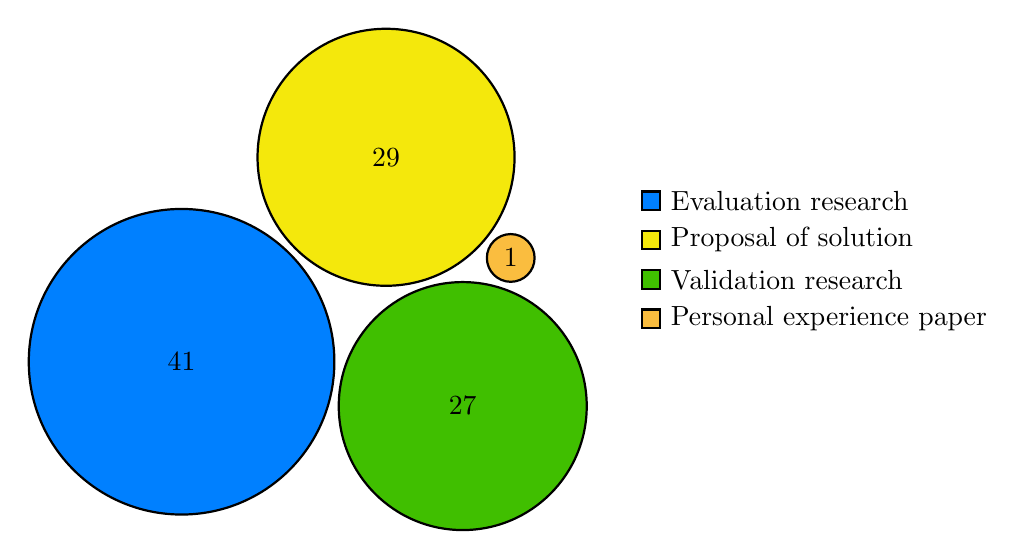
\begin{tikzpicture}
    \pie[cloud, text=legend, sum=98, color={blue!50!cyan, yellow!95!black, red!25!green, magenta!25!yellow}]
    {41/Evaluation research, 29/Proposal of solution, 27/Validation research, 1/Personal experience paper}
  \end{tikzpicture}
  \caption{Number of articles by type of study}
  \label{kuvaTyypit}
\end{figure}

The most common category of research is evaluation research (41 out of 98, 41.84\%).
Evaluation research papers present studies where the software application was tested in a realistic environment.
Studies with tests in a laboratory environment are validation research papers, and
there are 27 such papers (27.55\%) within the articles.
Proposal of solution papers with little reported evidence are also frequent with 29 results (29.59\%).
There is one personal experience paper (1.02\%), \textcite{xu2014rove},
which focuses on depicting the lessons learned during the process of software development
rather than the software application or testing it.

The first inclusion criterion of this thesis demands the included literature to present or evaluate
a singular software that was developed or will be developed for intellectually or developmentally disabled users.
This criterion alone excludes a large number of studies that consider software for these users.
Studies that present multiple software applications, or only demonstrate good software development practices
within this context, would undeniably be connected to the subject and informative,
but narrowly out of scope for this thesis.
The first criterion excludes philosophical papers, opinion papers, and most personal experience papers,
but this thesis cannot and will not claim their contents trivial nor negligible.


\section{Disabilities of intended users} % kysymys 3

Figure~\ref{kuvaVammat} depicts all of the disabilities extracted from the articles.
The disabilities are divided into two groups: nonspecific and specific disabilities.
Nonspecific disabilities refer to disabilities that serve as umbrella terms for specific disabilities
(e.g. intellectual disability is an umbrella term that includes Down syndrome), and they are shown in blue.
Specific disabilities are shown in yellow.
Seven articles mentioned two different disabilities, and thus the total number
of mentioned disabilities in Figure~\ref{kuvaVammat} is 105.
The acronym CCN refers to \textit{complex communication needs}, IDD to \textit{intellectual and developmental disabilities},
and ASD to \textit{Autism spectrum disorders}.
The figure shows that two disabilities are mentioned significantly more than the rest:
ASD with 44 mentions, and intellectual disability with 32 mentions.

\begin{figure}[thb]
  \centering
  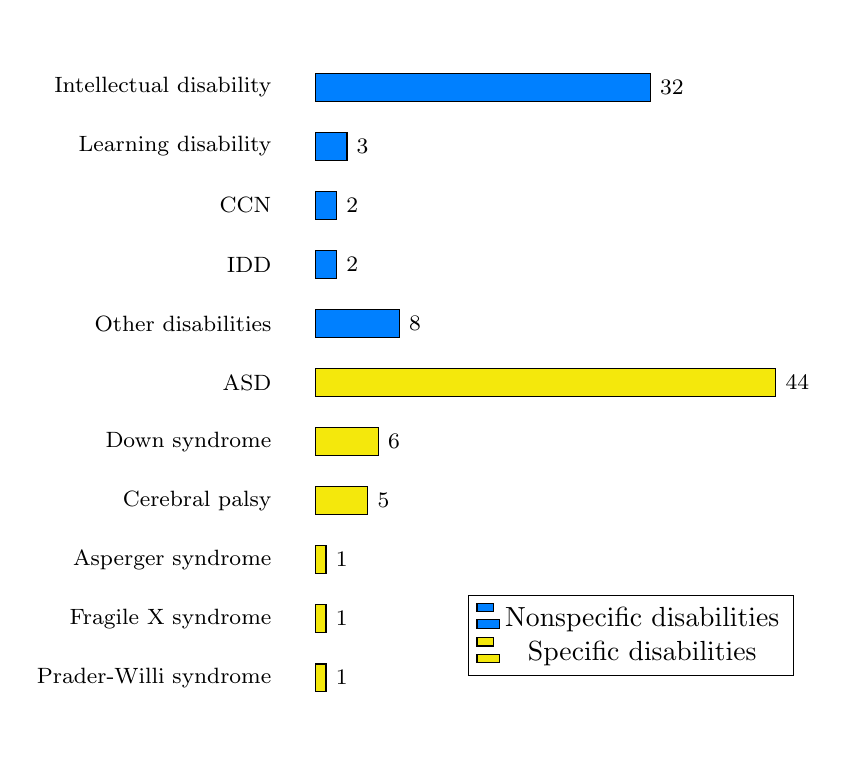
\begin{tikzpicture}
    \begin{axis} [
        xbar,
        nodes near coords,
        every node near coord/.append style={font=\footnotesize, anchor=west},
        y=0.75cm,
        bar width=10pt,
        width=\axisdefaultwidth,
        y axis line style = {opacity=0},
        axis x line = none,
        tickwidth = 0pt,
        yticklabel style = {font=\footnotesize},
        legend style={
            at={(0.95,0.2)},
          },
        symbolic y coords = {Prader-Willi syndrome, Fragile X syndrome, Asperger syndrome, Cerebral palsy, Down syndrome, ASD, Other disabilities, IDD, CCN, Learning disability, Intellectual disability},
        ytick = {Prader-Willi syndrome, Fragile X syndrome, Asperger syndrome, Cerebral palsy, Down syndrome, ASD, Other disabilities, IDD, CCN, Learning disability, Intellectual disability},
      ]
      \addplot[bar shift=0pt, fill=blue!50!cyan] coordinates { (32,Intellectual disability) (3,Learning disability) (2,CCN) (2,IDD) (8,Other disabilities) };
      \addplot[bar shift=0pt, fill=yellow!95!black] coordinates { (44,ASD) (6,Down syndrome) (5,Cerebral palsy) (1,Asperger syndrome) (1,Fragile X syndrome) (1,Prader-Willi syndrome) };
      \legend{Nonspecific disabilities, Specific disabilities}
    \end{axis}
  \end{tikzpicture}
  \caption{Number of articles by disability of intended users}
  \label{kuvaVammat}
\end{figure}

The nonspecific disabilities (intellectual disability, learning disability, CCN, IDD, and other disabilities)
have 47 mentions (44.76\%), and specific disabilities (ASD, Down syndrome, cerebral palsy,
Asperger syndrome, fragile X syndrome, Prader-Willi syndrome) have 58 mentions (55.24\%).
Despite only searching for the broader terms \textit{intellectual disability} and \textit{developmental disability}
in the literature searches, these terms have 35 mentions (32 for intellectual disability, one for developmental disability,
and two for IDD), which is 33.33\% of all 105 mentions.
The reasons for this seem two-fold: features of the used search engines affect the articles that are shown,
and the broader term may have been mentioned in the article (as a keyword or otherwise) without
it being the intended disability of users that was extracted as an answer to this research question.
Especially Google Scholar might include articles in the search results that do not strictly match the search terms,
instead prioritizing search results that other users have expressed interest towards.

Autism spectrum disorders have the most mentions though they were not included in the search terms.
Please note that here ASD includes all mentions of Autism and Autism spectrum disorders,
but not Asperger syndrome. For the purposes of this thesis, ASD is considered a specific disability
(under the umbrella term developmental disability),
although ASD could be considered an umbrella term itself.
Redefining ASD or merging all existing definitions is outside the scope of this thesis.

The disabilities in Figure~\ref{kuvaVammat} are the exact terms used in the articles, with the exception of
one article which speaks of \textit{cerebral paralysis} and four articles which speak of
\textit{intellectually challenged people} (one article), \textit{mental disability} (one article) and
\textit{mental retardation} (two articles). These are categorized as
\textit{cerebral palsy} and \textit{intellectual disability}, respectively.

The ``other disabilities'' in Figure~\ref{kuvaVammat} cover eight nonspecific disabilities,
with one mention each. These disabilities are:
cognitive impairments, developmental disability, hidden disabilities, motor disabilities,
neurodevelopmental disorders, physical disability, special educational needs, and verbal communication disorders.
\textit{Cognitive impairments} include for example traumatic brain injury, intellectual disability,
schizophrenia and Down syndrome \parencite{chang2012feasibility}.
\textcite{poyade2019isensevr} use the term \textit{hidden disabilities} for ASD,
Asperger syndrome, acute sensory hypersensitivity, post-traumatic stress disorder,
bipolar disorder, anxiety disorders and other general mental health conditions considered to be
within the spectrum of neurodevelopmental disorders.
\textit{Special educational needs} is used by \textcite{kraleva2017childibu} in relation to
children with speech, musculoskeletal system, or cognitive development disorders,
such as children with ASD and/or intellectual disabilities.
Adhering to explicitly stated information, the above terms could not be grouped with
other named disabilities, even though they have direct connections with each other.


\section{Ages of intended users} % kysymys 4

Figure~\ref{kuvaIät} presents the intended users of the software, divided into broad categories
based on the terms used in the 98 articles.
Children are the most popular age group with 57 articles (58.16\%).
Most studies (77 out of 98) specify some age group that their software targets,
while the rest (21 articles) do not. This group of unspecified ages consists
of studies where the focus is on aiding people regardless of age,
or where the test participants or intended users are a certain age
but the software application is stated to suit others as well.

\begin{figure}[thb]
  \centering
  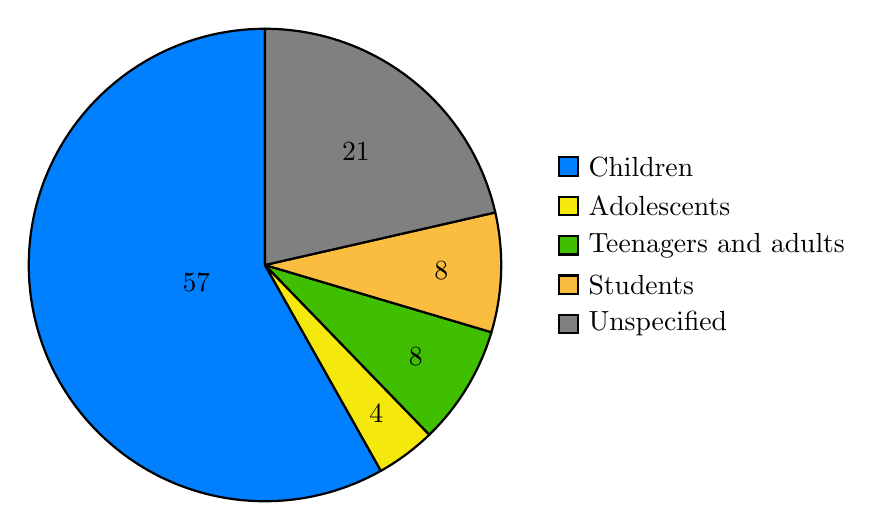
\begin{tikzpicture}
    \pie [rotate=90, text=legend, sum=98, color={blue!50!cyan, yellow!95!black, red!25!green, magenta!25!yellow, gray}]
    {57/Children, 4/Adolescents, 8/Teenagers and adults, 8/Students, 21/Unspecified}
  \end{tikzpicture}
  \caption{Number of articles by broad age groups of intended users}
  \label{kuvaIät}
\end{figure}

``Students'' is a group of its own because of two articles where
the software applications are proclaimed as targeting students, but the test participants
are 8--68, or 19--41 years old, respectively. For the remaining six studies in the
student category, ages are either unmentioned or within the range of 8--17 years.

% CHILDREN 57 kpl, includes young children (2), preschoolers (1), children (53) and school children (1)
% ADOLESCENTS 4 kpl, includes children and adolescents (1), young people (1), adolescents (2)
% TEENAGERS AND ADULTS 8 kpl, includes teenagers and young adults (1), young adults (3), adults (4)
% STUDENTS 8 kpl (sekavat iät)
% UNSPECIFIED 21 kpl

\begin{table}[h]
  \centering
  \begin{tabular}{|l|p{5cm}|c|l|}
    \hline
    \textbf{Broad age group}              & \textbf{Age group}                   & \textbf{Results} & \textbf{Age range} \\ \hline
    \multirow{4}{*}{Children}             & Young children                       & 2                & 0--6 years         \\
                                          & Preschoolers                         & 1                & 2--6 years         \\
                                          & Children                             & 53               & 0--12 years        \\
                                          & School children                      & 1                & K12 students       \\ \hline
    \multirow{3}{*}{Adolescents}          & Children and adolescents             & 1                & 11--15 years       \\
                                          & Young people                         & 1                & 14--18 years       \\
                                          & Adolescents                          & 2                & 13--18 years       \\ \hline
    \multirow{3}{*}{Teenagers and adults} & Teenagers and young adults           & 1                & 16--18 years       \\
                                          & Young adults                         & 3                & 17--35 years       \\
                                          & Adults                               & 4                & 18+ years          \\ \hline
    Students                              & Students                             & 8                & 8--68 years        \\ \hline
    \multicolumn{2}{|l|}{\textbf{Total}}  & \multicolumn{2}{l|}{\textbf{~~~~77}}                                         \\ \hline% sorry not sorry for the ''~~~~''
  \end{tabular}
  \caption{Extracted age groups of intended users}
  \label{agegroups}
\end{table}

A more detailed list of age groups can be found in Table~\ref{agegroups},
which includes the 77 articles that specify an age range they target.
The ``age group'' column represents the terms that were extracted from the articles,
while the ``broad age group'' column indicates how the age groups were simplified for Figure~\ref{kuvaIät}.
Values for the last column, ``age range'', are either age ranges that were specified as being targeted,
if the information was available, or the ages of test participants.
Not all articles specify an age range for their targeted age group or even their test participants.
For example, the age group ``children'' only has five articles of 53 where an age range is presented.
When there are multiple results specifying age ranges in the same age group,
the ranges are combined with a logical ``or'' operation.
There is some overlap of age ranges between different broad age groups,
most notably the student group spanning all the way from children to adults,
but also the ``adolescents'' group sharing 16--18-year-olds with the ``teenagers and adults'' group.

While children are the most targeted age group, users aged 18 or above have little attention.
Adults have nine mentions (combining age groups ``young adults'' with three articles, ``adults'' with four,
and the two articles from ``students'' where the age range was notably large), comprising only 9.18\%
of articles, excluding the software applications that are aimed at all ages.


\section{Platforms of applications} % kysymys 5

Figure~\ref{kuvaAlustat} shows the platform distribution of the software applications,
and different colors show how many applications are meant to be used with an additional tool or device.
According to the first inclusion criterion of this thesis, only applications developed for
the five platforms shown in the figure are considered.
Only applications to be used by a disabled user are included, although some of
the articles also present an another application for a guardian, teacher or tutor, either for managing
the application of a disabled user or gaining information about their progress.

Of the 98 articles, 94 are included in the figure.
There are four results where the platform information could not be extracted.
They either do not mention the platform, or no prototype has been made.
Please note that even articles where no prototype has yet been made are included in this figure
if they clearly indicate that the application will be only made available on a specific platform.
In two articles the software is presented as having both a mobile and a PC version.
These articles count towards both platforms' totals, making the total of all mentions 96.
The platforms in descending order of popularity are:
mobile (36 mentions), PC (27 mentions), web (16 mentions), VR (13 mentions), and AR (4 mentions).

\begin{figure}[thb]
  \centering
  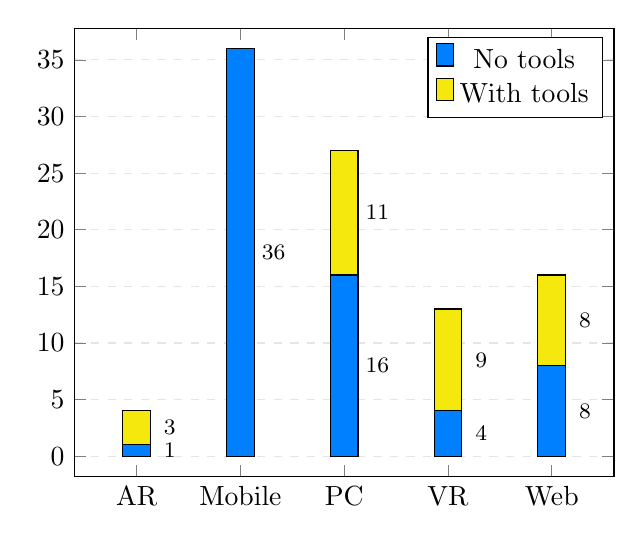
\begin{tikzpicture}
    \begin{axis}[
        ybar stacked,
        bar width=10pt,
        nodes near coords,%näyttää lukumäärät
        every node near coord/.append style={xshift=12pt,font=\footnotesize},
        enlarge x limits=0.15,
        enlarge y limits=0.05,
        symbolic x coords={AR, Mobile, PC, VR, Web},
        xtick=data,%tämä toimii näin vain koska jälkimmäisessä addplotissa ei ole uusia x-koordinaatteja
        ymin=0,
        ytick={0,5,...,35},
        grid style={dashed, draw=gray!20},
        ymajorgrids=true,
      ]
      \addplot [fill=blue!50!cyan] coordinates {(AR,1) (Mobile,36) (PC,16) (VR,4) (Web,8)};%plain
      \addplot [fill=yellow!95!black] coordinates {(AR,3) (Mobile,0) (PC,11) (VR,9) (Web,8)};%with a tool
      \legend{No tools,With tools}
    \end{axis}
  \end{tikzpicture}
  \caption{Number of articles by software platform}
  \label{kuvaAlustat}
\end{figure}

The ``mobile'' category encompasses a variety of devices,
including at least smart devices (phones, tablets, and watches),
PDAs (personal digital assistant), and so called ``pocket PCs''.
Articles are categorized as VR if they clearly speak of virtual environments
even when they do not specify the equipment used with the software application.

As is evident from Figure~\ref{kuvaAlustat}, a total of 31 software applications from
multiple platforms are meant to be used with an additional tool or a specific device.
Table~\ref{tools} gives an overview of the tools and devices, divided into three groups:
\begin{enumerate}
  \item The software application is recommended to be used with a specific device.
  \item The software application is used with a physical tool.
  \item The software application is used with a software tool.
\end{enumerate}

\begin{table}[h]
  \centering
  \begin{tabular}{|c|p{3cm}|c|c|c|c|>{\bfseries}r|}
    \hline
                                      & \textbf{Device or tool} & \textbf{AR} & \textbf{PC} & \textbf{VR} & \textbf{Web} & Total \\ \hline
    \multirow{2}{*}{\textit{Group 1}} & laptop                  & 1           & -           & -           & -            & 1     \\
                                      & mobile                  & 2           & -           & 2           & 7            & 11    \\ \hline
    \multirow{7}{*}{\textit{Group 2}} & custom tool             & -           & 3           & -           & -            & 3     \\
                                      & driving controller      & -           & -           & 1           & -            & 1     \\
                                      & EEG device              & -           & 1           & -           & -            & 1     \\
                                      & eye tracker             & -           & 1           & -           & -            & 1     \\
                                      & Kinect                  & -           & 4           & 4           & -            & 8     \\
                                      & Leap Motion             & -           & -           & 2           & 1            & 3     \\
                                      & RFID reader             & -           & 1           & -           & -            & 1     \\ \hline
    \textit{Group 3}                  & GlovePIE                & -           & 1           & -           & -            & 1     \\ \hline
                                      & \textbf{Total}          & \textbf{3}  & \textbf{11} & \textbf{9}  & \textbf{8}   & 31    \\ \hline
  \end{tabular}
  \caption{Tangible and intangible tools to be used with the applications}
  \label{tools}
\end{table}

The most popular physical tool is the Kinect sensor, having eight mentions out of 18 physical tools.
Other mentions are more evenly dispersed, most tools having only one mention.
The second most popular physical tools are custom tools and the Leap Motion
sensor, both with three mentions.
There are three different custom-made physical tools mentioned in the results:
a device with coloured buttons, a pressure pad mat, and a pressure sensing keypad.
They are all meant to be used with a PC software.
The software tool and majority of the physical tools (16 out of 18, excluding the EEG device, and eye tracker)
affect how input of the user is obtained, as motor difficulties may prevent
a user with IDD from effectively utilizing traditional mouse interactions.
Motion controls (Kinect, Leap Motion) are a popular user input style with physical tools,
and many of the other tools (custom tools, driving controller, RFID reader) either
are or resemble real life objects.

In addition to the 36 applications developed for the mobile platform, another 11 software applications
from other platforms are meant to be used on or with a mobile device,
meaning 47 software from 98 articles (47.96\%) have a direct connection to the mobile platform.
Multiple studies have found benefits to using mobile technology with intellectually or developmentally disabled users.
\textcite{artoni2013portable} characterized the mobile platform as being cheap, flexible, simple to use, and easily transportable.
\textcite{mcnaughton2013} found that mobile technologies present many potential benefits to the use and development of
augmentative and alternative communication technologies,
such as increased awareness and social acceptance, increased adoption of the technologies,
and greater diffusion of research and development.
Additionally, a review of 34 studies of people with developmental disabilities using touchscreen mobile devices found
that interventions using small-n designs were effective (25 studies), while group designs (five studies) and
case studies (four studies) both found positive effects for touch device use~\parencite{stephenson2015}.


\section{Purposes of applications} % kysymys 6

Figure~\ref{kuvaTarkoitukset} lists all of the different purposes the software applications from the
98 articles are made for. The most popular three purposes are
games (26 articles, 26.53\%), learning applications (23 articles, 23.47\%),
and AAC (augmentative and alternative communication) applications (12 articles, 12.24\%).
The purposes encompass, for example, teaching the user various things, and
helping the user communicate, travel, work, and otherwise live their life.

\begin{figure}[thb]
  \centering
  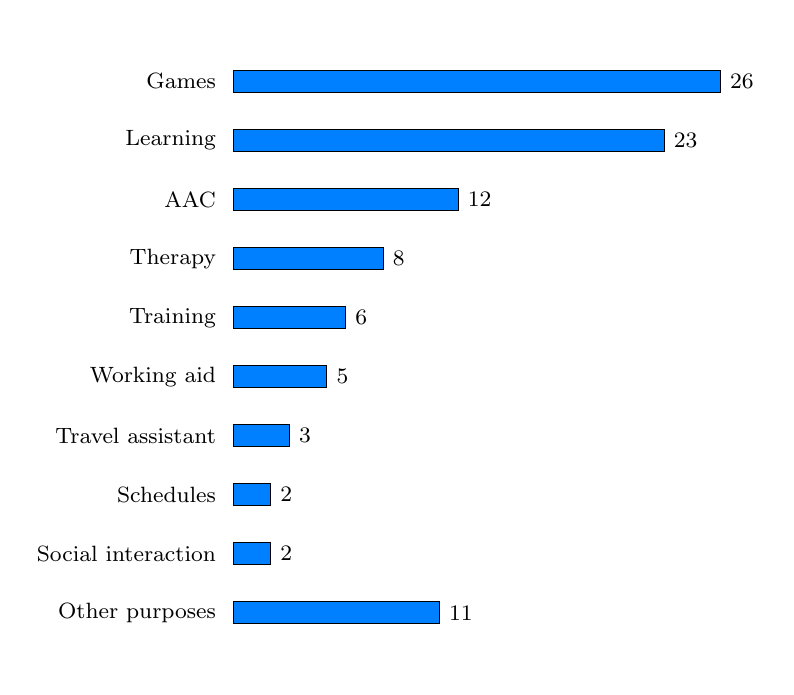
\begin{tikzpicture}
    \begin{axis} [
        xbar,
        nodes near coords,
        every node near coord/.append style={font=\footnotesize, anchor=west},
        y=0.75cm,
        bar width=8pt,
        width=\axisdefaultwidth,
        y axis line style = {opacity=0},
        axis x line = none,
        tickwidth = 0pt,
        yticklabel style = {font=\footnotesize},
        symbolic y coords = {Other purposes, Social interaction, Schedules, Travel assistant, Working aid, Training, Therapy, AAC, Learning, Games},
        ytick = data,
      ]
      \addplot[bar shift=0pt, fill=blue!50!cyan] coordinates { (26,Games) (23,Learning) (12,AAC) (8,Therapy) (6,Training) (5,Working aid) (3,Travel assistant) (2,Schedules) (2,Social interaction) (11,Other purposes) };
    \end{axis}
  \end{tikzpicture}
  \caption{Number of articles by purpose of the software application}
  \label{kuvaTarkoitukset}
\end{figure}

The purpose categories emerge from the articles, and especially the ``games'' category has overlap with the others.
Of the 26 game applications, seven are \textit{learning games}, six are \textit{serious games},
five are \textit{educational games}, and two are \textit{therapeutic games}.
A further three games are, with one mention each, a \textit{cognitive training game},
a \textit{collaborative game}, and a \textit{training game}.
Only three software applications in the games category have no other objective attached to them.

The eight therapy applications encompass seven different therapy forms.
Two applications are made to assist in ABA intervention~\parencite{artoni2013portable, artoni2018technology}.
Speech, music, physical, and exposure therapy all have their own application within the articles.
A VR application virtualizes dolphin therapy to increase the non-verbal communication of the user~\parencite{cai2013}.
The last therapy application is a multisensory environment (Snoezelen environment) application.

The other purposes in Figure~\ref{kuvaTarkoitukset} refer to 11
software applications with purposes that cannot be included in the other categories.
Those applications are:
\begin{itemize}
  \item Aid for pretend play,
  \item Alternative text entry with brain-computer interface,
  \item Decision support tool for clinical trial consent,
  \item Driving VR environment,
  \item Gesture recognition system,
  \item Instructional tool for individualized teaching,
  \item Job interest assessment system,
  \item Multimedia platform,
  \item Planning aid for setting goals,
  \item Social story comprehension checking application, and
  \item User's needs, abilities and preferences identifying application for participatory design.
\end{itemize}

Appendix~\ref{appendixC} lists all skills that the software applications from the articles claim to improve.
A total of 61 articles out of 98 (62.2\%) assert that their application improves, trains or teaches one or multiple skills.
These 61 articles come from several purpose categories (see Figure~\ref{kuvaTarkoitukset}).
The trained skills are extracted from the articles like answers to research questions:
adhering to information that is explicitly mentioned.
For the sake of brevity, some skills are combined, provided they appear to have the same content
or they can be united under a common term.

The skills listed in Appendix~\ref{appendixC} are divided into six categories
that emerge from the extracted skills:
cognitive, communicative, language, life, mathematical, and social skills.
Cognitive skills include skills regarding executive functions such as learning, memory, and attention.
Communicative skills include communication and speech fluency, while
language skills involve reading, writing, and vocabulary.
Life skills encompass a wide range of skills, including self-care, independence,
and more specific matters such as history, piano playing, or pre-vocational skills.
Mathematical skills involve numeracy and calculation.
Social skills is again more broad, concerning matters such as collaboration,
recognition of emotions or facial expressions,
empathy, and other-awareness.

Of all the different skills that the applications in accepted articles exercise,
life skills are the most popularly improved skills with 22 mentions,
and cognitive skills come second with 17 mentions.
Social skills have 15, language skills 13, and communicative skills 11 mentions.
Mathematical skills have eight mentions.
Please note that these categories do not all share the same scope,
as for example mathematical skills have a very narrow scope while
life skills encompass a wide range of skills.


%############################################
%                                    Johtopäätökset
%############################################
\chapter{Conclusion}

This mapping study examined 98 articles that presented software applications
developed for people with intellectual or developmental disabilities,
published as journal articles or conference papers in 2010--2019.
The amount of literature was small, but showed signs of growth through the decade
rising from two accepted articles in 2010 to 15 accepted articles in 2019.
Types of research present in the articles were
evaluation research (41.84\%),
proposal of solution (29.59\%),
validation research (27.55\%), and
personal experience paper (1.02\%),
using the classification system by~\textcite{wieringa2006requirements}.
The remaining categories, philosophical papers and opinion papers,
were not present in the accepted articles due to the inclusion criteria of this study.

The 98 articles were dispersed through 80 different publication forums.
The largest number of articles to arise from a single forum was four.
The number of forums being very high, it seems there was no
devoted forum for publishing studies specifically about software applications
for people with IDD. The studies were instead published in disability-specific
forums, or forums regarding human-computer interaction, accessibility,
or educational technology.

Most common disabilities of the intended users of these applications
were Autism spectrum disorders (44 out of 105) and intellectual disability (32 out of 105),
and both of these disabilities had an estimated prevalence of around 1\% of general population~\parencite{dsm5}.
Of all mentioned disabilities, 44.76\% were nonspecific (e.g. intellectual disability),
and 55.24\% were specific (e.g. Down syndrome),
when Autism/ASD was considered a specific disability under the umbrella term developmental disability.
ASD could also be considered nonspecific, which would render
86.67\% of the mentioned disabilities nonspecific.

Children with IDD were clearly the most popular age group,
intended users of these applications being children in 58.16\% of the articles.
Early intervention is often cited as more effective and an important part
of rehabilitation~\parencite[e.g.][]{almeida2019, artoni2018technology},
which may partly explain the frequency of publications about children.
There were only eight applications aimed at teenagers and adults within the 98 articles of this study.
The software needs and desires of teenagers and adults with IDD may differ
from those of a child, and therefore those age groups warrant further study.

The mobile platform was the most popular platform,
encompassing 47.96\% of the articles (36 mobile applications and 11 applications from other
platforms meant to be used with a mobile device).
The dominance of mobile device use is unsurprising, considering
that many studies have reported positive effects of touchscreen mobile device use
by people with developmental disabilities~\parencite{stephenson2015}.
This thesis also found that 18 of 98 applications were meant to be used with a physical tool.
The Kinect sensor was the most popular physical tool, with the Leap Motion sensor and
custom tools as second. One application was meant to be used with a software tool, GlovePIE.
GlovePIE and 16 out of 18 physical tools concerned user input,
helping to overcome the motor difficulties some people with IDD present.

The most popular three purposes of the software applications in a classification that emerged from the articles
were games (26.53\%), learning (23.47\%), and augmentative and alternative communication (12.24\%).
The games category had some overlap with other categories, including learning, therapy, and training,
implying that gaming could be used as a tool in aiding people with IDD.
A significant portion (62.2\%) of the articles claimed that their software application
improved one or multiple skills of the user. Life skills were the most popularly improved skills.
Appendix~\ref{appendixC} lists all improved skills with numbers of mentions.

This mapping study assessed 2978 search results from five search engines.
After re-reviewing 159 potential articles, the accepted 98 articles were found.
The overall acception rate of articles was 3.29\%,
varying from Google Scholar's 2.15\% to IEEE Xplore's 51.85\%.
Having such a low rate of accepted articles may indicate that the used search terms
were either unsuitable for the search engines or inadequately refined.
Assessing an excessive number of search results enabled refining the scope of this thesis
during literature searches, but with sufficient planning some unnecessary work
could have been avoided.

\textcite{kitchenham2011} presented potential problems in conducting a mapping study
as a Master's student, including time and effort restrictions and insufficient rigor.
With these potential problems in mind, this thesis has the following limitations:
the articles were assessed for inclusion by a single author,
the data extracted by a single author,
and time restrictions hastened the mapping process.
In an effort to convince the reader of sufficient rigor,
Chapter~\ref{method} described in detail the mapping process as it was
conducted within this thesis.
Most notably this thesis considered multiple additional parts of papers somewhat
uncharacteristically to a mapping study, which according to~\textcite{petersen2008}
increases the validity of results.

This thesis aimed to fill a gap in the scientific literature of software developed for
people with intellectual or developmental disabilities.
As a limited search conducted for similar secondary studies found only
one other mapping study but multiple literature reviews
(findings listed in Appendix~\ref{appendixD}),
it was concluded that the research area would benefit from a systematic mapping study.
However, two mapping studies with different scopes hardly
render the area fully saturated, and therefore more mapping studies
can and should be made of the area.

The primary motivation behind this thesis was the thought
that everyone should have the right to learn.
As Finland is one of the many countries to sign and ratify the
Convention on the Rights of Persons with Disabilities~\parencite{unitednations},
this thesis may be considered an attempt to better the access to suitable
software applications that persons with disabilities should have
as part of their human rights.
Chapter~\ref{softat} displayed multiple examples of applications
developed for intellectually or developmentally disabled people that could help them learn,
gain access to therapy, or lead more independent lives by training necessary skills.
The examples will hopefully serve as inspiration to caretakers and teachers of people with IDD.


\printbibliography %LÄHTEET

\appendix
\section{Accepted articles} \label{appendixA}

\begin{footnotesize}
  The following table lists the 98 accepted articles of this mapping study.
  The articles are sorted first by ascending year, then alphabetically by author name.
\end{footnotesize}

\begin{longtable}{|>{\scriptsize}l|>{\scriptsize}p{3cm}|>{\scriptsize}p{8cm}|>{\scriptsize}p{2.4cm}|}
  \hline
  \textbf{Year} & \textbf{Authors}                                                     & \textbf{Title}                                                                                                                                                                               & \textbf{Type of research}  \\
  \hline
  \endfirsthead
  \multicolumn{4}{c}{\textit{Accepted results - Continued from previous page}}                                                                                                                                                                                                                                     \\
  \hline
  \endhead
  \multicolumn{4}{c}{\textit{Continued on next page}}                                                                                                                                                                                                                                                              \\
  \endfoot
  \hline
  \endlastfoot

  2010          & Colomo-Palacios, Paniagua-Martín, García-Crespo, Ruiz-Mezcua         & Technology enhanced learning for people with intellectual disabilities and cerebral paralysis: The MAS platform                                                                              & Proposal of solution       \\ \hline
  2010          & Kuan, Jiar, Supriyanto                                               & Language assessment and training support system (LATSS) for down syndrome children under 6 years old                                                                                         & Validation research        \\ \hline
  2011          & Alja'am, Jaoua, Alhazbi, Hassan et al.                               & An assistive computerized system for children with moderate intellectual and learning disabilities                                                                                           & Proposal of solution       \\ \hline
  2011          & Anwar, Rahman, Ferdous, Anik et al.                                  & A Computer Game Based Approach for Increasing Fluency in the Speech of the Autistic Children                                                                                                 & Validation research        \\ \hline
  2011          & Brown, McHugh, Standen, Evett et al.                                 & Designing location-based learning experiences for people with intellectual disabilities and additional sensory impairments                                                                   & Validation research        \\ \hline
  2011          & De Leo, Gonzales, Battagiri, Leroy                                   & A Smart-Phone Application and a Companion Website for the Improvement of the Communication Skills of Children with Autism: Clinical Rationale, Technical Development and Preliminary Results & Evaluation research        \\ \hline
  2011          & Idwan, Aldajeha, Matar, Mutlaq                                       & Building hand activities application for cerebral palsy children                                                                                                                             & Proposal of solution       \\ \hline
  2011          & Sahin, Cimen                                                         & An Interactive Attention Board: Improving the Attention of Individuals with Autism and Mental Retardation                                                                                    & Evaluation research        \\ \hline
  2012          & Chang, Chen, Chou                                                    & A feasibility study of enhancing independent task performance for people with cognitive impairments through the use of a handheld location-based prompting system                            & Evaluation research        \\ \hline
  2012          & Da Silva, Gonçalves, Guerreiro, Silva                                & A Web-based Application to Address Individual Interests of Children with Autism Spectrum Disorders                                                                                           & Proposal of solution       \\ \hline
  2012          & Keskinen, Heimonen, Turunen, Rajaniemi et al.                        & SymbolChat: A flexible picture-based communication platform for users with intellectual disabilities                                                                                         & Evaluation research        \\ \hline
  2012          & Muñoz, Barcelos, Noël, Kreisel                                       & Development of Software that Supports the Improvement of the Empathy in Children with Autism Spectrum Disorder                                                                               & Evaluation research        \\ \hline
  2013          & Aliee, Jomhari, Rezaei, Alias                                        & The Effectiveness of Managing Split Attention Among Autistic Children Using Computer Based Intervention                                                                                      & Validation research        \\ \hline
  2013          & Artoni, Buzzi, Buzzi, Fenili et al.                                  & A portable application for supporting ABA intervention                                                                                                                                       & Validation research        \\ \hline
  2013          & Bekele, Young, Zheng, Zhang et al.                                   & A step towards adaptive multimodal virtual social interaction platform for children with autism                                                                                              & Proposal of solution       \\ \hline
  2013          & Brown, Standen, Saridaki, Shopland et al.                            & Engaging students with intellectual disabilities through games based learning and related technologies                                                                                       & Evaluation research        \\ \hline
  2013          & Burke, Allen, Howard, Downey et al.                                  & Tablet-based video modeling and prompting in the workplace for individuals with autism                                                                                                       & Evaluation research        \\ \hline
  2013          & Cai, Chia, Thalmann, Kee et al.                                      & Design and development of a virtual dolphinarium for children with autism                                                                                                                    & Validation research        \\ \hline
  2013          & Farias, Cunha, Souza-Júnior, Jacinto                                 & Designing of a TEACCH-based software prototype for assisting in literacy of children with autism spectrum disorders                                                                          & Proposal of solution       \\ \hline
  2013          & Husni                                                                & Mobile applications BIUTIS: Let's study vocabulary learning as a media for children with autism                                                                                              & Proposal of solution       \\ \hline
  2013          & Li, Ip                                                               & AIMtechKinect: A Kinect Based Interaction-Oriented Gesture Recognition System Designed for Students with Severe Intellectual Disabilities                                                    & Evaluation research        \\ \hline
  2013          & Lorenzo, Pomares, Lledó                                              & Inclusion of immersive virtual learning environments and visual control systems to support the learning of students with Asperger syndrome                                                   & Validation research        \\ \hline
  2013          & Puspitasari, Ummah, Pambudy                                          & KIDEA: An innovative computer technology to improve skills in children with intelectual disability using Kinect sensor                                                                       & Proposal of solution       \\ \hline
  2013          & Saleh, Aljaam, El Saddik                                             & An integrated e-learning system for MID and MLD children in Qatar                                                                                                                            & Proposal of solution       \\ \hline
  2013          & Saleh, Aljaam, Karime, El Saddik                                     & An edutainment system for assisting qatari children with moderate intellectual and learning disability through exerting physical activities                                                  & Evaluation research        \\ \hline
  2013          & Vullamparthi, Nelaturu, Mallaya, Chandrasekhar                       & Assistive learning for children with autism using augmented reality                                                                                                                          & Proposal of solution       \\ \hline
  2014          & Baldassarri, Rubio, Azpiroz, Cerezo                                  & AraBoard: A multiplatform alternative and augmentative communication tool                                                                                                                    & Evaluation research        \\ \hline
  2014          & Bargagna, Bozza, Buzzi, Buzzi et al.                                 & Computer-Based Cognitive Training in Adults with Down’s Syndrome                                                                                                                             & Validation research        \\ \hline
  2014          & Christinaki, Vidakis, Triantafyllidis                                & A novel educational game for teaching emotion identification skills to preschoolers with autism diagnosis                                                                                    & Validation research        \\ \hline
  2014          & Holt, Yuill                                                          & Facilitating Other-Awareness in Low-Functioning Children with Autism and Typically-Developing Preschoolers Using Dual-Control Technology                                                     & Evaluation research        \\ \hline
  2014          & Ribeiro, de Araujo, Raposo                                           & ComFiM: a cooperative serious game to encourage the development of communicative skills between children with autism                                                                         & Validation research        \\ \hline
  2014          & Xu, Zhang, Yagovkin, Maniero et al.                                  & Rove n Rave™ development: a partnership between the university and the disability service provider to build a social website for people with an intellectual disability                      & Personal experience papers \\ \hline
  2015          & Babic, Slivar, Car, Podobnik                                         & Prototype-driven software development process for augmentative and alternative communication applications                                                                                    & Proposal of solution       \\ \hline
  2015          & Banire, Jomhari, Ahmad                                               & Visual Hybrid Development Learning System (VHDLS) Framework for Children with Autism                                                                                                         & Evaluation research        \\ \hline
  2015          & Benda, Šmejkalová                                                    & Web Interface for Education of Mentally Disabled Persons for Work in Horticulture                                                                                                            & Evaluation research        \\ \hline
  2015          & Benda, Ulman, Šmejkalová                                             & Augmented Reality As a Working Aid for Intellectually Disabled Persons For Work in Horticulture                                                                                              & Evaluation research        \\ \hline
  2015          & Borblik, Shabalina, Kultsova, Pidoprigora et al.                     & Assistive technology software for people with intellectual or development disabilities: Design of user interfaces for mobile applications                                                    & Proposal of solution       \\ \hline
  2015          & Castelhano, Roque                                                    & The “Malha” project: A game design proposal for multisensory stimulation environments                                                                                                        & Proposal of solution       \\ \hline
  2015          & Colpani, Homem                                                       & An innovative augmented reality educational framework with gamification to assist the learning process of children with intellectual disabilities                                            & Proposal of solution       \\ \hline
  2015          & El-Seoud, Karkar, Al Ja'am, Karam                                    & A Pictorial Mobile Application for Improving Communication Skills in Non-Verbal Autism                                                                                                       & Proposal of solution       \\ \hline
  2015          & Freina, Bottino, Ott, Costa                                          & Social Empowerment of Intellectually Impaired through a Cloud Mobile System                                                                                                                  & Evaluation research        \\ \hline
  2015          & Hatzigiannakoglou                                                    & Junk-Food Destroyer: Helping adolescents with Down syndrome to understand healthy eating through serious game                                                                                & Proposal of solution       \\ \hline
  2015          & Kaneyama, Goto, Nishino                                              & Methodology for developing ICT based course material for children with a developmental disability based on EPISODE                                                                           & Proposal of solution       \\ \hline
  2015          & Perhakaran, Yusof, Rusli, Yusoff et al.                              & SnoezelenCAVE: Virtual reality CAVE Snoezelen framework for Autism spectrum disorders                                                                                                        & Proposal of solution       \\ \hline
  2015          & Saturno, Ramirez, Conte, Farhat et al.                               & An augmentative and alternative communication tool for children and adolescents with cerebral palsy                                                                                          & Evaluation research        \\ \hline
  2016          & de Oliveira, Fernandes, Pinto, Pinheiro et al.                       & Novel Virtual Environment for Alternative Treatment of Children with Cerebral Palsy                                                                                                          & Proposal of solution       \\ \hline
  2016          & Eliçin, Tunalı                                                       & Effectiveness of Tablet Computer Use in Achievement of Schedule-Following Skills by Children with Autism Using Graduated Guidance                                                            & Evaluation research        \\ \hline
  2016          & Kamaruzaman, Rani, Nor, Azahari                                      & Developing User Interface Design Application for Children with Autism                                                                                                                        & Proposal of solution       \\ \hline
  2016          & Kultsova, Romanenko, Zhukova, Usov et al.                            & Assistive mobile application for support of mobility and communication of people with IDD                                                                                                    & Proposal of solution       \\ \hline
  2016          & Paulino, Amaral, Amaral, Reis et al.                                 & Professor Piano: a music application for people with intellectual disabilities                                                                                                               & Validation research        \\ \hline
  2016          & Piki, Markou, Vasiliou                                               & Learning Through Play: The Role of Learning and Engagement Theory in the Development of Educational Games for Intellectually Challenged Children                                             & Proposal of solution       \\ \hline
  2016          & Santos, Breda, Almeida                                               & Learning Environment for Autism Spectrum Disorders: a universal approach to the promotion of mathematical reasoning                                                                          & Validation research        \\ \hline
  2016          & Sulaiman, Ghazali                                                    & Learning through Playing for Children with Cerebral Palsy                                                                                                                                    & Evaluation research        \\ \hline
  2016          & Wade, Zhang, Bian, Fan et al.                                        & A Gaze-Contingent Adaptive Virtual Reality Driving Environment for Intervention in Individuals with Autism Spectrum Disorders                                                                & Validation research        \\ \hline
  2016          & Welton, Brown, Evett, Sherkat                                        & A brain-computer interface for the Dasher alternative text entry system                                                                                                                      & Validation research        \\ \hline
  2016          & Wilson, Sitbon, Brereton, Johnson et al.                             & Put yourself in the picture': designing for futures with young adults with intellectual disability                                                                                           & Evaluation research        \\ \hline
  2017          & Bourazeri, Bellamy-Wood, Arnab                                       & EnCity: A serious game for empowering young people with Down's syndrome                                                                                                                      & Proposal of solution       \\ \hline
  2017          & Felix, Mena, Ostos, Maestre                                          & A pilot study of the use of emerging computer technologies to improve the effectiveness of reading and writing therapies in children with Down syndrome                                      & Evaluation research        \\ \hline
  2017          & Hara, Bigham                                                         & Introducing people with ASD to crowd work                                                                                                                                                    & Evaluation research        \\ \hline
  2017          & Javadi, Ghazvini, Dianat                                             & Mobile Speech Therapy Application Using Speech Processing for Intellectually Disabled Children                                                                                               & Evaluation research        \\ \hline
  2017          & Kraleva                                                              & ChilDiBu - A mobile application for Bulgarian Children with special educational needs                                                                                                        & Proposal of solution       \\ \hline
  2017          & Pradi, Bellon, Silva, Dória et al.                                   & Visual computing tool for training recognition and production of facial expressions by children with autism                                                                                  & Evaluation research        \\ \hline
  2017          & Rodríguez-Sedano, Conde-González, Fernández-Llamas, Esteban-Costales & The Use of a New Visual Language as a Supporting Resource for People with Intellectual Disabilities                                                                                          & Evaluation research        \\ \hline
  2017          & Segatto, Melo,da Silva                                               & Proposal of an educational game for improvement of cognitive performance of intellectually disabled people                                                                                   & Evaluation research        \\ \hline
  2017          & Tashnim, Nowshin, Akter, Das                                         & Interactive interface design for learning numeracy and calculation for children with autism                                                                                                  & Proposal of solution       \\ \hline
  2017          & Tsiopela, Jimoyiannis                                                & Pre-vocational skills laboratory: designing interventions to improve employment skills for students with autism spectrum disorders                                                           & Validation research        \\ \hline
  2017          & Wojciechowski, Al-Musawi                                             & Assisstive technology application for enhancing social and language skills of young children with autism                                                                                     & Evaluation research        \\ \hline
  2017          & Zaki, Islam, Uddin, Tumpa et al.                                     & Towards developing a learning tool for children with autism                                                                                                                                  & Validation research        \\ \hline
  2018          & Alexopoulou, Kastampolidou, Bobori                                   & Educational Multi-Sensory Game for Students with Mental Retardation                                                                                                                          & Proposal of solution       \\ \hline
  2018          & Artoni, Bastiani, Buzzi, Buzzi et al.                                & Technology-enhanced ABA intervention in children with autism: a pilot study                                                                                                                  & Evaluation research        \\ \hline
  2018          & Baratè, Elia, Ludovico, Oriolo                                       & The Leap Motion Controller in Clinical Music Therapy: A Computer-Based Approach to Intellectual and Motor Disabilities                                                                       & Evaluation research        \\ \hline
  2018          & Davies, Stock, Davies, Wehmeyer                                      & A cloud-supported app for providing self-directed, localized job interest assessment and analysis for people with intellectual disability                                                    & Evaluation research        \\ \hline
  2018          & Davies, Stock, Herold, Wehmeyer                                      & GeoTalk: a GPS-Enabled Portable Speech Output Device for People with Intellectual Disability                                                                                                 & Evaluation research        \\ \hline
  2018          & Dragomir, Manches, Fletcher-Watson, Pain                             & Facilitating Pretend Play in Autistic Children: Results from an Augmented Reality App Evaluation                                                                                             & Evaluation research        \\ \hline
  2018          & Ekin, Çağiltay, Karasu                                               & Usability study of a smart toy on students with intellectual disabilities                                                                                                                    & Validation research        \\ \hline
  2018          & Furberg, Ortiz, Moultrie, Raspa et al.                               & A digital decision support tool to enhance decisional capacity for clinical trial consent: design and development                                                                            & Validation research        \\ \hline
  2018          & Ip, Wong, Chan, Byrne et al.                                         & Enhance emotional and social adaptation skills for children with autism spectrum disorder: A virtual reality enabled approach                                                                & Validation research        \\ \hline
  2018          & Khowaja, Al-Thani, Salim                                             & Vocabulary Learning of Children With Autism Spectrum Disorder (ASD): From the Development to an Evaluation of Serious Game Prototype                                                         & Validation research        \\ \hline
  2018          & Line, Loureiro, Prates                                               & Musical App in Hypersensitivity to Sounds and Neurodevelopmental Disorders: Applicable Strategies                                                                                            & Proposal of solution       \\ \hline
  2018          & Muñoz, Becerra, Noël, Camblor et al.                                 & Design, Implementation and Evaluation of a Learning Object that Supports the Mathematics Learning in Children with Autism Spectrum Disorders.                                                & Evaluation research        \\ \hline
  2018          & Munoz, Morales, Villarroel, Quezada et al.                           & Developing a Software That Supports the Improvement of the Theory of Mind in Children With Autism Spectrum Disorder                                                                          & Evaluation research        \\ \hline
  2018          & Pavlov, Castro, Chukanska, Molina et al.                             & Mobile Graphical User Interface with People with Verbal Communication Disorders                                                                                                              & Proposal of solution       \\ \hline
  2018          & Zhang, Fu, Swanson, Weitlauf et al.                                  & Design and Evaluation of a Collaborative Virtual Environment (CoMove) for Autism Spectrum Disorder Intervention                                                                              & Validation research        \\ \hline
  2019          & Ajisafe, Bethi, King, Katangur                                       & Development and Usability of a Low-Cost Kinect Game to Promote Movement Competence in Children with and Without Intellectual Disability                                                      & Validation research        \\ \hline
  2019          & Almeida, Silva, Theodório, Silva et al.                              & ALTRIRAS: A Computer Game for Training Children with Autism Spectrum Disorder in the Recognition of Basic Emotions                                                                           & Validation research        \\ \hline
  2019          & Camargo, Carvalho, Barros, Barros et al.                             & Improving Usability of a Mobile Application for Children with Autism Spectrum Disorder Using Heuristic Evaluation                                                                            & Validation research        \\ \hline
  2019          & Cano, García-Tejedor, Alonso-Fernández, Fernández-Manjón             & Game Analytics Evidence-Based Evaluation of a Learning Game for Intellectual Disabled Users                                                                                                  & Evaluation research        \\ \hline
  2019          & Carniel, Berkenbrock, Berkenbrock, da Costa et al.                   & Supporting the Dialog of People With Intellectual Disabilities Through Augmentative and Alternative Communication                                                                            & Evaluation research        \\ \hline
  2019          & Chan, Sato-Shimokawara, Bai, Yukiharu et al.                         & A Context-Aware Augmentative and Alternative Communication System for School Children With Intellectual Disabilities                                                                         & Evaluation research        \\ \hline
  2019          & Chebli, Lanovaz, Dufour                                              & Comparison of tablet-delivered and instructor-delivered teaching on receptive identification in children with autism spectrum disorders                                                      & Evaluation research        \\ \hline
  2019          & Constantin, Georgiou, Alexandru, Korte                               & $S^2C^2$: Toward an App to Support Social Story™ Comprehension Checking in Children with ASD                                                                                                 & Validation research        \\ \hline
  2019          & Ferreira, Castro                                                     & Identifying User Preferences Through an Application for Autistic Children Using Inclusive Design Models                                                                                      & Evaluation research        \\ \hline
  2019          & Kang, Chang                                                          & Using a motion-controlled game to teach four elementary school children with intellectual disabilities to improve hand hygiene                                                               & Evaluation research        \\ \hline
  2019          & Politis, Olivia, Olivia                                              & Empowering autistic adults through their involvement in the development of a virtual world                                                                                                   & Validation research        \\ \hline
  2019          & Poyade, Morris, Taylor, Portela                                      & iSenseVR: bringing VR exposure therapy outside the laboratory                                                                                                                                & Evaluation research        \\ \hline
  2019          & Rezae, McMeekin, Tan, Krishna et al.                                 & Public transport planning tool for users on the autism spectrum: from concept to prototype                                                                                                   & Proposal of solution       \\ \hline
  2019          & Robb, Waller, Woodcock                                               & Developing a task switching training game for children with a rare genetic syndrome linked to intellectual disability                                                                        & Evaluation research        \\ \hline
  2019          & Sullivan, Wilson, Saldaña                                            & Development of a gaze contingent method for auditory threshold evaluation in non-verbal ASD children                                                                                         & Validation research        \\
\end{longtable}


\section{Excluded potential articles} \label{appendixB}

\begin{footnotesize}
  The following table lists the 61 potential articles that were excluded during the second phase of the literature search.
  The articles are sorted first by ascending year, then alphabetically by author name.
\end{footnotesize}

\begin{longtable}{|>{\scriptsize}l|>{\scriptsize}p{3cm}|>{\scriptsize}p{10.4cm}|}
  \hline
  \textbf{Year} & \textbf{Authors}                                             & \textbf{Title}                                                                                                                                                                                                                 \\
  \hline
  \endfirsthead
  \multicolumn{3}{c}{\textit{ Excluded results - Continued from previous page}}                                                                                                                                                                                                                                 \\
  \hline
  \endhead
  \multicolumn{3}{c}{\textit{Continued on next page}}                                                                                                                                                                                                                                                           \\
  \endfoot
  \hline
  \endlastfoot

  1994          & Greenwood, Carta, Kamps, Terry et al.                        & Development and validation of standard classroom observation systems for school practitioners: Ecobehavioral Assessment Systems Software (EBASS)                                                                               \\ \hline
  1999          & Hagiwara, Smith Myles                                        & A multimedia social story intervention: Teaching skill to children with autism                                                                                                                                                 \\ \hline
  2004          & Stock, Davies, Wehmeyer                                      & Internet-Based Multimedia Tests and Surveys for Individuals with Intellectual Disabilities                                                                                                                                     \\ \hline
  2005          & Riffel, Wehmeyer, Turnbull, Lattimore et al.                 & Promoting Independent Performance of Transition-Related Tasks Using a Palmtop PC-based Self-Directed Visual and Auditory Prompting System                                                                                      \\ \hline
  2009          & Bauchet, Pigot, Giroux, Lussier-Desrochers et al.            & Designing judicious interactions for cognitive assistance: the acts of assistance approach                                                                                                                                     \\ \hline
  2009          & Francis, Balbo, Firth                                        & Towards co-design with users who have autism spectrum disorders                                                                                                                                                                \\ \hline
  2010          & Ferreras, Belda, Barberà, Poveda et al.                      & PDA Software Aimed at Improving Workplace Adaptation for People with Cognitive Disabilities                                                                                                                                    \\ \hline
  2010          & Hofmann, Hoppe, Jantke                                       & The Need for Special Games for Gamers with Special Needs                                                                                                                                                                       \\ \hline
  2010          & Paniagua-Martin, Colomo-Palacios, Garcia-Crespo, Ruiz-Mezcua & MAS: building an educational platform for people with intellectual disabilities and cerebral paralysis                                                                                                                         \\ \hline
  2011          & Aljaam, Jaoua, AlHazbi, Hasnah et al.                        & An Assistive Computerized System with Tangible User Interfaces for Children with Moderate Intellectual and Learning Disabilities                                                                                               \\ \hline
  2011          & Artoni, Buzzi, Buzzi, Fenili et al.                          & Accessible Education for Autistic Children: ABA-Based Didactic Software                                                                                                                                                        \\ \hline
  2011          & Da Silva, Simões, Da Silva, Guerreiro et al.                 & Rapid application development using web technologies. An application to communicative competence promotion of children with ASD                                                                                                \\ \hline
  2011          & Saleh, Aljaam, Jaoua, Elsaddik                               & An Arabic-Based Tutorial System for Children with Special Needs                                                                                                                                                                \\ \hline
  2011          & Travers, Higgins, Pierce, Boone et al.                       & Emergent Literacy Skills of Preschool Students with Autism: A Comparison of Teacher-led and Computer-Assisted Instruction                                                                                                      \\ \hline
  2011          & Valeria, Lau                                                 & Learn with Me: Collaborative Virtual Learning for the Special Children                                                                                                                                                         \\ \hline
  2012          & Aljaam, Mwinyi, Elzeiny, Dandashi et al.                     & An ontology-based system to dynamically extract multimedia elements for children's tutorials                                                                                                                                   \\ \hline
  2012          & Hailpern, Harris, Botz, Birman et al.                        & Designing visualizations to facilitate multisyllabic speech with children with autism and speech delays                                                                                                                        \\ \hline
  2012          & Hernández, Zorrilla, Zapirain                                & Management Platform to Support Intellectually Disabled People Daily Tasks Using Android Smartphones                                                                                                                            \\ \hline
  2012          & Keay-bright, Howarth                                         & Is simplicity the key to engagement for children on the autism spectrum?                                                                                                                                                       \\ \hline
  2012          & Silva, Andrade, Santana                                      & Performance of disabled students in mathematical activities in the adapted gcompris software system                                                                                                                            \\ \hline
  2012          & Zamfir, Tedesco, Reichow                                     & Handheld “app” offering visual support to students with autism spectrum disorders (ASDs)                                                                                                                                       \\ \hline
  2013          & Buzzi, Buzzi, Rapisarda, Senette et al.                      & Teaching low-functioning autistic children: ABCD SW                                                                                                                                                                            \\ \hline
  2013          & Vismara, Mccormick, Young, Nadhan et al.                     & Preliminary Findings of a Telehealth Approach to Parent Training in Autism                                                                                                                                                     \\ \hline
  2014          & Chatzara, Karagiannidis, Mavropoulou, Stamatis               & Digital Storytelling for Children with Autism: Software Development and Pilot Application                                                                                                                                      \\ \hline
  2014          & El-Seoud, Karkar, Al Ja'am, Karam                            & A pictorial mobile-based communication application for non-verbal people with autism                                                                                                                                           \\ \hline
  2014          & Gómez-Martínez, Gonzalez-Cabero, Merseguer                   & Performance assessment of an architecture with adaptative interfaces for people with special needs                                                                                                                             \\ \hline
  2014          & Lee, Choi, Song, Shin                                        & Dreamware: Edutainment system for children with developmental disability                                                                                                                                                       \\ \hline
  2014          & Picardo, Metson, Hoda, Amor et al.                           & Towards designing assistive software applications for discrete trial training                                                                                                                                                  \\ \hline
  2014          & Silva, Raposo, Suplino                                       & PAR: A Collaborative Game for Multitouch Tabletop to Support Social Interaction of Users with Autism                                                                                                                           \\ \hline
  2014          & Tsiopela, Jimoyiannis                                        & Pre-vocational Skills Laboratory: Development and Investigation of a Web-based Environment for Students with Autism                                                                                                            \\ \hline
  2014          & Wade, Bian, Zhang, Swanson et al.                            & Design of a Virtual Reality Driving Environment to Assess Performance of Teenagers with ASD                                                                                                                                    \\ \hline
  2015          & Dekelver, Daems, Solberg, Bosch et al.                       & Viamigo: A digital travel assistant for people with intellectual disabilities: Modeling and design using contemporary intelligent technologies as a support for independent traveling of people with intellectual disabilities \\ \hline
  2015          & Dekelver, Kultsova, Shabalina, Borblik et al.                & Design of mobile applications for people with intellectual disabilities                                                                                                                                                        \\ \hline
  2015          & Groba, Pereira, Nieto, Pousada et al.                        & ASD Module: a software to support the personal autonomy in the daily life of children with autism spectrum disorder                                                                                                            \\ \hline
  2015          & Hani, Abu-Wandi                                              & DISSERO Mobile Application for AUTISTIC Children's                                                                                                                                                                             \\ \hline
  2015          & Ito, Nozawa, Miyairi, Takaishi                               & Educational Support for Children with Special Needs: K-12 SNE Kids Touch                                                                                                                                                       \\ \hline
  2015          & Santos, Breda, Almeida                                       & Brief Report: Preliminary Proposal of a Conceptual Model of a Digital Environment for Developing Mathematical Reasoning in Students with Autism Spectrum Disorders                                                             \\ \hline
  2015          & Wainer, Ingersoll                                            & Increasing Access to an ASD Imitation Intervention Via a Telehealth Parent Training Program                                                                                                                                    \\ \hline
  2016          & Cano, Fernández-Manjón, García-Tejedor                       & Downtown, a Subway Adventure: Using Learning Analytics to Improve the Development of a Learning Game for People with Intellectual Disabilities                                                                                 \\ \hline
  2016          & Daems, Bosch, Solberg, Dekelver et al.                       & AbleChat: Development of a chat app with pictograms for People with Intellectual Disabilities                                                                                                                                  \\ \hline
  2016          & Hamidy, Fathoni, Pu, Ilham                                   & Android Maze Game for Children as an Autism Therapy                                                                                                                                                                            \\ \hline
  2016          & Reardon, Wright, Cihak, Parker                               & Intelligent context-aware augmented reality to teach students with intellectual and developmental disabilities                                                                                                                 \\ \hline
  2016          & Ribu, Patel                                                  & Developing a User-Centred Planning Tool for Young Adults with Development Disorders: A Research-Based Teaching Project.                                                                                                        \\ \hline
  2016          & Tsikinas, Xinogalos, Satratzemi                              & Review on serious games for people with intellectual disabilities and autism                                                                                                                                                   \\ \hline
  2017          & Chuchra, Sharma                                              & PROPOSING MMABOAR: MIND MAP APPLICATION BASED ON AUGMENTED REALITY                                                                                                                                                             \\ \hline
  2017          & Esposito, Sloan, Tancredi, Gerardi et al.                    & Using Tablet Applications for Children With Autism to Increase Their Cognitive and Social Skills                                                                                                                               \\ \hline
  2017          & Karanfiller, Göksu, Yurtkan                                  & A Mobile Application Design for Students Who Need Special Education                                                                                                                                                            \\ \hline
  2017          & Rocha, Carvalho, Bessa, Reis et al.                          & Usability evaluation of navigation tasks by people with intellectual disabilities: a Google and SAPO comparative study regarding different interaction modalities                                                              \\ \hline
  2017          & Sadry, Ismail                                                & AutiShapes: Learning shapes game for autistic children on mobile application                                                                                                                                                   \\ \hline
  2017          & Shin, Min, Rayz, Matson                                      & Semantic Knowledge-Based Language Education Device for Children with Developmental Disabilities                                                                                                                                \\ \hline
  2018          & Afra, Bruggers, Sweney, Fagatele et al.                      & Mobile Software as a Medical Device (SaMD) for the Treatment of Epilepsy: Development of Digital Therapeutics Comprising Behavioral and Music-Based Interventions for Neurological Disorders                                   \\ \hline
  2018          & Larco, Montenegro, Diaz, Luján-Mora                          & Underlying Quality Factors in Spanish Language Apps for People with Disabilities                                                                                                                                               \\ \hline
  2018          & Larco, Montenegro, Luján-Mora                                & Quality improvement criteria of apps in Spanish for people with disabilities                                                                                                                                                   \\ \hline
  2018          & Lazar, Woglom, Chung, Schwartz et al.                        & Co-design process of a smart phone app to help people with down syndrome manage their nutritional habits                                                                                                                       \\ \hline
  2018          & Pashapoor, Kashani-Vahid, Hakimirad                          & Effectiveness of Cognitive Computer games on Attention Span of Students with Intellectual Disability                                                                                                                           \\ \hline
  2018          & Stancheva-Popkostadinova, Andreeva                           & PILOTING INTERACTIVE KINECT-BASED GAME IN CHILDREN WITH DISABILITIES.                                                                                                                                                          \\ \hline
  2018          & Zubair, Brown, Hughes-Roberts, Bates                         & Evaluating the Accessibility of Scratch for Children with Cognitive Impairments                                                                                                                                                \\ \hline
  2019          & Akin, Gokturk                                                & Comparison of the Theory of Mind Tests on the Paper, 2D Touch Screen and Augmented Reality Environments on the Students With Neurodevelopmental Disorders                                                                      \\ \hline
  2019          & Crowell, Mora-Guiard, Pares                                  & Structuring collaboration: Multi-user full-body interaction environments for children with Autism Spectrum Disorder                                                                                                            \\ \hline
  2019          & Kadam, Ghodke, Sadhukhan                                     & Hand Gesture Recognition Software Based on Indian Sign Language                                                                                                                                                                \\ \hline
  2019          & Khullar, Singh, Bala                                         & IoT based Assistive Companion for Hypersensitive Individuals (ACHI) with Autism Spectrum Disorder                                                                                                                              \\
\end{longtable}

\section{Skills the applications aim to improve} \label{appendixC}

\begin{footnotesize}
  The following tables contain skills that 61 out of 98 accepted articles
  explicitly mentioned to improve with their software applications.
  The skills are divided into six categories that emerged from the skills:
  cognitive, communicative, language, life, mathematical, and social skills.
  The numbers on the right reflect the number of mentions a particular skill had.

  The skills were extracted adhering to information explicitly mentioned
  in the articles. For the sake of brevity, some skills were combined,
  provided the skills appeared the same or could be united under a
  common term. In many cases, one article claimed to improve multiple skills.
\end{footnotesize}

\begin{tabular}{cc}
  \textbf{Cognitive skills}  & \textbf{Communicative skills} \\
  %cognitive skills table
  \begin{tabular}{|>{\footnotesize}p{4.5cm}|>{\footnotesize\centering\arraybackslash}p{1.5cm}|}
    \hline
    Attention                                         & 1           \\ \hline
    Cognitive performance                             & 1           \\ \hline
    Cognitive skills                                  & 2           \\ \hline
    Executive functions                               & 1           \\ \hline
    Learning capabilities                             & 4           \\ \hline
    Memorization skills                               & 2           \\ \hline
    Memory                                            & 1           \\ \hline
    Task switching                                    & 1           \\ \hline
    Thinking skills                                   & 2           \\ \hline
    Understanding                                     & 2           \\ \hline
    \multicolumn{1}{|r|}{\footnotesize\textbf{Total}} & \textbf{17} \\ \hline
  \end{tabular} &
  %communicative skills table
  \begin{tabular}{|>{\footnotesize}p{4.5cm}|>{\footnotesize\centering\arraybackslash}p{1.5cm}|}
    \hline
    Communication                                     & 3           \\ \hline
    Communication capabilities                        & 1           \\ \hline
    Communication skills                              & 4           \\ \hline
    Communicative competences                         & 1           \\ \hline
    Nonverbal communication                           & 1           \\ \hline
    Speech fluency                                    & 1           \\ \hline
    \multicolumn{1}{|r|}{\footnotesize\textbf{Total}} & \textbf{11} \\ \hline
    \multicolumn{2}{c}{}                                            \\%näillä samalle tasolle kuin vierekkäinen taulukko
    \multicolumn{2}{c}{}                                            \\%näyttää pahalta, mutta tuntuu hyvältä
    \multicolumn{2}{c}{}                                            \\%(ja myös näyttää hyvältä pdf:ssä)
    \multicolumn{2}{c}{}                                            \\
  \end{tabular}                                 \\
\end{tabular}


\begin{tabular}{cc}
  \textbf{Language skills}   & \textbf{Life skills} \\
  %language skills table
  \begin{tabular}{|>{\footnotesize}p{4.5cm}|>{\footnotesize\centering\arraybackslash}p{1.5cm}|}
    \hline
    English alphabet                                  & 1           \\ \hline
    Hiragana                                          & 1           \\ \hline
    Language skills                                   & 2           \\ \hline
    Letters                                           & 1           \\ \hline
    Literacy                                          & 1           \\ \hline
    One-word concepts                                 & 1           \\ \hline
    Quran                                             & 2           \\ \hline
    Reading                                           & 1           \\ \hline
    Vocabulary                                        & 2           \\ \hline
    Writing                                           & 1           \\ \hline
    \multicolumn{1}{|r|}{\footnotesize\textbf{Total}} & \textbf{13} \\ \hline
    \multicolumn{2}{c}{}                                            \\
    \multicolumn{2}{c}{}                                            \\
    \multicolumn{2}{c}{}                                            \\
  \end{tabular} &
  %life skills table
  \begin{tabular}{|>{\footnotesize}p{4.5cm}|>{\footnotesize\centering\arraybackslash}p{1.5cm}|}
    \hline
    Colors                                            & 1           \\ \hline
    Daily life concepts                               & 1           \\ \hline
    General knowledge                                 & 1           \\ \hline
    Hand hygiene                                      & 1           \\ \hline
    Hand-eye coordination                             & 1           \\ \hline
    Healthy eating                                    & 2           \\ \hline
    History                                           & 1           \\ \hline
    Independence                                      & 4           \\ \hline
    Independent travel                                & 5           \\ \hline
    Life skills                                       & 1           \\ \hline
    Motor skills                                      & 2           \\ \hline
    Music (piano)                                     & 1           \\ \hline
    Pre-vocational skills                             & 1           \\ \hline
    \multicolumn{1}{|r|}{\footnotesize\textbf{Total}} & \textbf{22} \\ \hline
  \end{tabular}                        \\
\end{tabular}


\begin{tabular}{cc}
  \textbf{Mathematical skills} & \textbf{Social skills} \\
  %mathematical skills table
  \begin{tabular}{|>{\footnotesize}p{4.5cm}|>{\footnotesize\centering\arraybackslash}p{1.5cm}|}
    \hline
    Calculation                                       & 1          \\ \hline
    Mathematical reasoning                            & 1          \\ \hline
    Mathematics                                       & 3          \\ \hline
    Numbers                                           & 1          \\ \hline
    Numeracy                                          & 2          \\ \hline
    \multicolumn{1}{|r|}{\footnotesize\textbf{Total}} & \textbf{8} \\ \hline
    \multicolumn{2}{c}{}                                           \\
    \multicolumn{2}{c}{}                                           \\
    \multicolumn{2}{c}{}                                           \\
    \multicolumn{2}{c}{}                                           \\
    \multicolumn{2}{c}{}                                           \\
    \multicolumn{2}{c}{}                                           \\
  \end{tabular}   &
  %social skills table
  \begin{tabular}{|>{\footnotesize}p{4.5cm}|>{\footnotesize\centering\arraybackslash}p{1.5cm}|}
    \hline
    Collaborative behaviors                           & 1           \\ \hline
    Emotional skills                                  & 1           \\ \hline
    Empathy                                           & 1           \\ \hline
    Other-awareness                                   & 1           \\ \hline
    Recognition and production of facial expressions  & 1           \\ \hline
    Recognition of emotions                           & 3           \\ \hline
    Social adaptation skills                          & 1           \\ \hline
    Social competences                                & 1           \\ \hline
    Social skills                                     & 4           \\ \hline
    Theory of Mind                                    & 1           \\ \hline
    \multicolumn{1}{|r|}{\footnotesize\textbf{Total}} & \textbf{15} \\ \hline
  \end{tabular}                            \\
\end{tabular}


\section{Similar secondary studies} \label{appendixD}

\begin{footnotesize}
  Scopus, January 11th 2020.
  Search term \textit{TITLE-ABS-KEY ( ( "mapping study"  OR  "literature review" )  AND  ( "autism"  OR  "developmental disability"
    OR  "intellectual disability" ) )  AND  ( LIMIT-TO ( LANGUAGE ,  "English" ) )  AND  ( LIMIT-TO ( SUBJAREA ,  "COMP" )
    OR  LIMIT-TO ( SUBJAREA ,  "ENGI" ) )} yielded 53 search results. The following 13 relevant literature reviews were found:

  \begin{compactenum}
    \item Abdo, M., Al Osman, H. (2019) Technology Impact on Reading and writing skills of children with autism: a systematic literature review. Health and Technology, 9 (5), pp. 725-735.
    \item Adnan, N.H., Ahmad, I., Abdullasim, N. (2018) Systematic review on augmented reality application for autism children. Journal of Advanced Research in Dynamical and Control Systems, 10 (11), pp. 26-32.
    \item Börjesson, P., Barendregt, W., Eriksson, E., Torgersson, O. (2015) Designing technology for and with developmentally diverse children - A systematic literature review. Proceedings of IDC 2015: The 14th International Conference on Interaction Design and Children, art. no. 2771848, pp. 79-88.
    \item Cano, A.R., García-Tejedor, Á.J., Fernández-Manjón, B. (2015) A literature Review of Serious games for intellectual Disabilities. Lecture Notes in Computer Science (including subseries Lecture Notes in Artificial Intelligence and Lecture Notes in Bioinformatics), 9307, pp. 560-563.
    \item Constain, G., Collazos, C., Moreira, F. (2018) Use of HCI for the development of emotional skills in the treatment of Autism Spectrum Disorder: A systematic review. Iberian Conference on Information Systems and Technologies, CISTI, 2018-June, pp. 1-6.
    \item Den Brok, W.L.J.E., Sterkenburg, P.S. (2015) Self-controlled technologies to support skill attainment in persons with an autism spectrum disorder and/or an intellectual disability: A systematic literature review. Disability and Rehabilitation: Assistive Technology, 10 (1), pp. 1-10.
    \item Goosen, L. (2019) Information systems and technologies opening new worlds for learning to children with autism spectrum disorders. Smart Innovation, Systems and Technologies, 111, pp. 134-143.
    \item Hong, T.S., Mohamaddan, S., Shazali, S.T.S., Mohtadzar, N.A.A., Bakar, R.A. (2016) A review on assistive tools for autistic patients. IECBES 2016 - IEEE-EMBS Conference on Biomedical Engineering and Sciences, art. no. 7843413, pp. 51-56.
    \item Jingga, F., Meyliana, Hidayanto, A.N., Prabowo, H. (2019) Computer human interaction research for children with autism spectrum disorder (ASD): A systematic literature review. International Journal of Mechanical Engineering and Technology, 10 (2), pp. 1610-1619.
    \item Park, J., Bouck, E., Duenas, A. (2019) The Effect of Video Modeling and Video Prompting Interventions on Individuals With Intellectual Disability: A Systematic Literature Review. Journal of Special Education Technology, 34 (1), pp. 3-16.
    \item Shoaib, M., Hussain, I., Mirza, H.T., Tayyab, M. (2017) The role of information and innovative technology for rehabilitation of children with Autism: A Systematic Literature Review. Proceedings of the 2017 17th International Conference on Computational Science and Its Applications, ICCSA 2017, art. no. 7999647.
    \item Tsikinas, S., Xinogalos, S. (2019) Studying the effects of computer serious games on people with intellectual disabilities or autism spectrum disorder: A systematic literature review. Journal of Computer Assisted Learning, 35 (1), pp. 61-73.
    \item Valencia, K., Rusu, C., Quiñones, D., Jamet, E. (2019) The impact of technology on people with autism spectrum disorder: A systematic literature review. Sensors (Switzerland), 19 (20), art. no. 4485.
  \end{compactenum}

  Google Scholar, January 11th 2020. Several search terms found the following nine secondary studies
  (eight literature reviews and one mapping study) that were relevant:
  \begin{compactenum}
    \item Ascari, R. E. D. O. S., Pereira, R., Silva, L. (2018) Mobile Interaction for Augmentative and Alternative Communication: a Systematic Mapping. SBC Journal on Interactive Systems, 9(2), 105-118.
    \item Baxter, S., Enderby, P., Evans, P. and Judge, S. (2012) Barriers and facilitators to the use of high‐technology augmentative and alternative communication devices: a systematic review and qualitative synthesis. International Journal of Language \& Communication Disorders, 47: 115-129.
    \item Gilson, C. B., Carter, E. W., Biggs, E. E. (2017) Systematic review of instructional methods to teach employment skills to secondary students with intellectual and developmental disabilities. Research and Practice for Persons with Severe Disabilities, 42(2), 89-107.
    \item Koumpouros, Y., Kafazis, T. (2019) Wearables and mobile technologies in Autism Spectrum Disorder interventions: A systematic literature review. Research in Autism Spectrum Disorders, 66, art. no. 101405.
    \item Lorah, E. R., Parnell, A., Whitby, P. S., Hantula, D. (2015) A systematic review of tablet computers and portable media players as speech generating devices for individuals with autism spectrum disorder. Journal of Autism and Developmental Disorders, 45(12), 3792-3804.
    \item Martins, F. R., Fernandes, F. G., Naves, E. L. M. (2019) Serious Games in Neurorehabilitation for People with Intellectual and Cognitive Impairments: A Systematic Study. In XXVI Brazilian Congress on Biomedical Engineering (pp. 359-364). Springer, Singapore.
    \item Morash-Macneil, V., Johnson, F., Ryan, J. B. (2018) A systematic review of assistive technology for individuals with intellectual disability in the workplace. Journal of Special Education Technology, 33(1), 15-26.
    \item Ramdoss, S., Lang, R., Fragale, C., Britt, C., O’Reilly, M., Sigafoos, J., ... Lancioni, G. E. (2012) Use of computer-based interventions to promote daily living skills in individuals with intellectual disabilities: A systematic review. Journal of Developmental and Physical Disabilities, 24(2), 197-215.
    \item Ramdoss, S., Lang, R., Mulloy, A., Franco, J., O’Reilly, M., Didden, R., Lancioni, G. (2011) Use of computer-based interventions to teach communication skills to children with autism spectrum disorders: A systematic review. Journal of Behavioral Education, 20(1), 55-76.
  \end{compactenum}
\end{footnotesize}

\end{document}
